% Options for packages loaded elsewhere
\PassOptionsToPackage{unicode}{hyperref}
\PassOptionsToPackage{hyphens}{url}
\PassOptionsToPackage{dvipsnames,svgnames,x11names}{xcolor}
%
\documentclass[
  11pt,
]{article}

\usepackage{amsmath,amssymb}
\usepackage{iftex}
\ifPDFTeX
  \usepackage[T1]{fontenc}
  \usepackage[utf8]{inputenc}
  \usepackage{textcomp} % provide euro and other symbols
\else % if luatex or xetex
  \usepackage{unicode-math}
  \defaultfontfeatures{Scale=MatchLowercase}
  \defaultfontfeatures[\rmfamily]{Ligatures=TeX,Scale=1}
\fi
\usepackage{lmodern}
\ifPDFTeX\else  
    % xetex/luatex font selection
    \setmainfont[]{Aptos}
\fi
% Use upquote if available, for straight quotes in verbatim environments
\IfFileExists{upquote.sty}{\usepackage{upquote}}{}
\IfFileExists{microtype.sty}{% use microtype if available
  \usepackage[]{microtype}
  \UseMicrotypeSet[protrusion]{basicmath} % disable protrusion for tt fonts
}{}
\makeatletter
\@ifundefined{KOMAClassName}{% if non-KOMA class
  \IfFileExists{parskip.sty}{%
    \usepackage{parskip}
  }{% else
    \setlength{\parindent}{0pt}
    \setlength{\parskip}{6pt plus 2pt minus 1pt}}
}{% if KOMA class
  \KOMAoptions{parskip=half}}
\makeatother
\usepackage{xcolor}
\setlength{\emergencystretch}{3em} % prevent overfull lines
\setcounter{secnumdepth}{5}
% Make \paragraph and \subparagraph free-standing
\makeatletter
\ifx\paragraph\undefined\else
  \let\oldparagraph\paragraph
  \renewcommand{\paragraph}{
    \@ifstar
      \xxxParagraphStar
      \xxxParagraphNoStar
  }
  \newcommand{\xxxParagraphStar}[1]{\oldparagraph*{#1}\mbox{}}
  \newcommand{\xxxParagraphNoStar}[1]{\oldparagraph{#1}\mbox{}}
\fi
\ifx\subparagraph\undefined\else
  \let\oldsubparagraph\subparagraph
  \renewcommand{\subparagraph}{
    \@ifstar
      \xxxSubParagraphStar
      \xxxSubParagraphNoStar
  }
  \newcommand{\xxxSubParagraphStar}[1]{\oldsubparagraph*{#1}\mbox{}}
  \newcommand{\xxxSubParagraphNoStar}[1]{\oldsubparagraph{#1}\mbox{}}
\fi
\makeatother


\providecommand{\tightlist}{%
  \setlength{\itemsep}{0pt}\setlength{\parskip}{0pt}}\usepackage{longtable,booktabs,array}
\usepackage{calc} % for calculating minipage widths
% Correct order of tables after \paragraph or \subparagraph
\usepackage{etoolbox}
\makeatletter
\patchcmd\longtable{\par}{\if@noskipsec\mbox{}\fi\par}{}{}
\makeatother
% Allow footnotes in longtable head/foot
\IfFileExists{footnotehyper.sty}{\usepackage{footnotehyper}}{\usepackage{footnote}}
\makesavenoteenv{longtable}
\usepackage{graphicx}
\makeatletter
\def\maxwidth{\ifdim\Gin@nat@width>\linewidth\linewidth\else\Gin@nat@width\fi}
\def\maxheight{\ifdim\Gin@nat@height>\textheight\textheight\else\Gin@nat@height\fi}
\makeatother
% Scale images if necessary, so that they will not overflow the page
% margins by default, and it is still possible to overwrite the defaults
% using explicit options in \includegraphics[width, height, ...]{}
\setkeys{Gin}{width=\maxwidth,height=\maxheight,keepaspectratio}
% Set default figure placement to htbp
\makeatletter
\def\fps@figure{htbp}
\makeatother

\usepackage{booktabs}
\usepackage{longtable}
\usepackage{array}
\usepackage{multirow}
\usepackage{wrapfig}
\usepackage{float}
\usepackage{colortbl}
\usepackage{pdflscape}
\usepackage{tabu}
\usepackage{threeparttable}
\usepackage{threeparttablex}
\usepackage[normalem]{ulem}
\usepackage{makecell}
\usepackage{xcolor}
\usepackage{pdfpages}
\usepackage{fontspec}
\usepackage[bottom]{footmisc}
\setmainfont{Aptos}[Path="C:/Users/ginow/AppData/Roaming/TinyTeX/texmf-dist/fonts/truetype/aptos/", Extension=".ttf"]
\usepackage{fancyhdr}
\pagestyle{fancy}
\fancyhf{}
\usepackage{xcolor}
\fancyhead[C]{\makebox[\textwidth]{\hspace*{-1cm}
\includegraphics[height=1.9cm]{../Logotipo ENADEL/encabezado_izquierda1.png} \hfill 
\includegraphics[height=1.5cm]{../Logotipo ENADEL/encabezado_derecha.png} \hspace*{-2cm}}}
\fancyfoot[L]{\vspace{5pt}Subsecretaría del Trabajo}
\cfoot{\thepage}
\setlength{\footskip}{10pt}
\setlength{\skip\footins}{15pt}
\setlength{\headheight}{3cm}
\setlength{\headsep}{0.5cm}
\setlength{\footskip}{25pt}
\renewcommand{\thefootnote}{\textcolor{gray}{\arabic{footnote}}}
\setlength{\skip\footins}{1.5em}
\floatplacement{figure}{H}
\floatplacement{table}{H}
\usepackage{geometry}
\geometry{ left=3cm, right=3cm, top=2.5cm, bottom=2.5cm }
\usepackage{placeins}
\usepackage{ragged2e}
\usepackage{float}
\usepackage{setspace}
\renewcommand{\familydefault}{\sfdefault}
\AtBeginDocument{\renewcommand{\baselinestretch}{1.5}\justifying}
\usepackage{pagecolor}
\makeatletter
\@ifpackageloaded{caption}{}{\usepackage{caption}}
\AtBeginDocument{%
\ifdefined\contentsname
  \renewcommand*\contentsname{Tabla de contenidos}
\else
  \newcommand\contentsname{Tabla de contenidos}
\fi
\ifdefined\listfigurename
  \renewcommand*\listfigurename{Listado de Figuras}
\else
  \newcommand\listfigurename{Listado de Figuras}
\fi
\ifdefined\listtablename
  \renewcommand*\listtablename{Listado de Tablas}
\else
  \newcommand\listtablename{Listado de Tablas}
\fi
\ifdefined\figurename
  \renewcommand*\figurename{Figura}
\else
  \newcommand\figurename{Figura}
\fi
\ifdefined\tablename
  \renewcommand*\tablename{Tabla}
\else
  \newcommand\tablename{Tabla}
\fi
}
\@ifpackageloaded{float}{}{\usepackage{float}}
\floatstyle{ruled}
\@ifundefined{c@chapter}{\newfloat{codelisting}{h}{lop}}{\newfloat{codelisting}{h}{lop}[chapter]}
\floatname{codelisting}{Listado}
\newcommand*\listoflistings{\listof{codelisting}{Listado de Listados}}
\makeatother
\makeatletter
\makeatother
\makeatletter
\@ifpackageloaded{caption}{}{\usepackage{caption}}
\@ifpackageloaded{subcaption}{}{\usepackage{subcaption}}
\makeatother

\ifLuaTeX
\usepackage[bidi=basic]{babel}
\else
\usepackage[bidi=default]{babel}
\fi
\babelprovide[main,import]{spanish}
\ifPDFTeX
\else
\babelfont{rm}[]{Aptos}
\fi
% get rid of language-specific shorthands (see #6817):
\let\LanguageShortHands\languageshorthands
\def\languageshorthands#1{}
\ifLuaTeX
  \usepackage{selnolig}  % disable illegal ligatures
\fi
\usepackage{bookmark}

\IfFileExists{xurl.sty}{\usepackage{xurl}}{} % add URL line breaks if available
\urlstyle{same} % disable monospaced font for URLs
\hypersetup{
  pdflang={es},
  colorlinks=true,
  linkcolor={blue},
  filecolor={Maroon},
  citecolor={Blue},
  urlcolor={Blue},
  pdfcreator={LaTeX via pandoc}}


\author{}
\date{}

\begin{document}

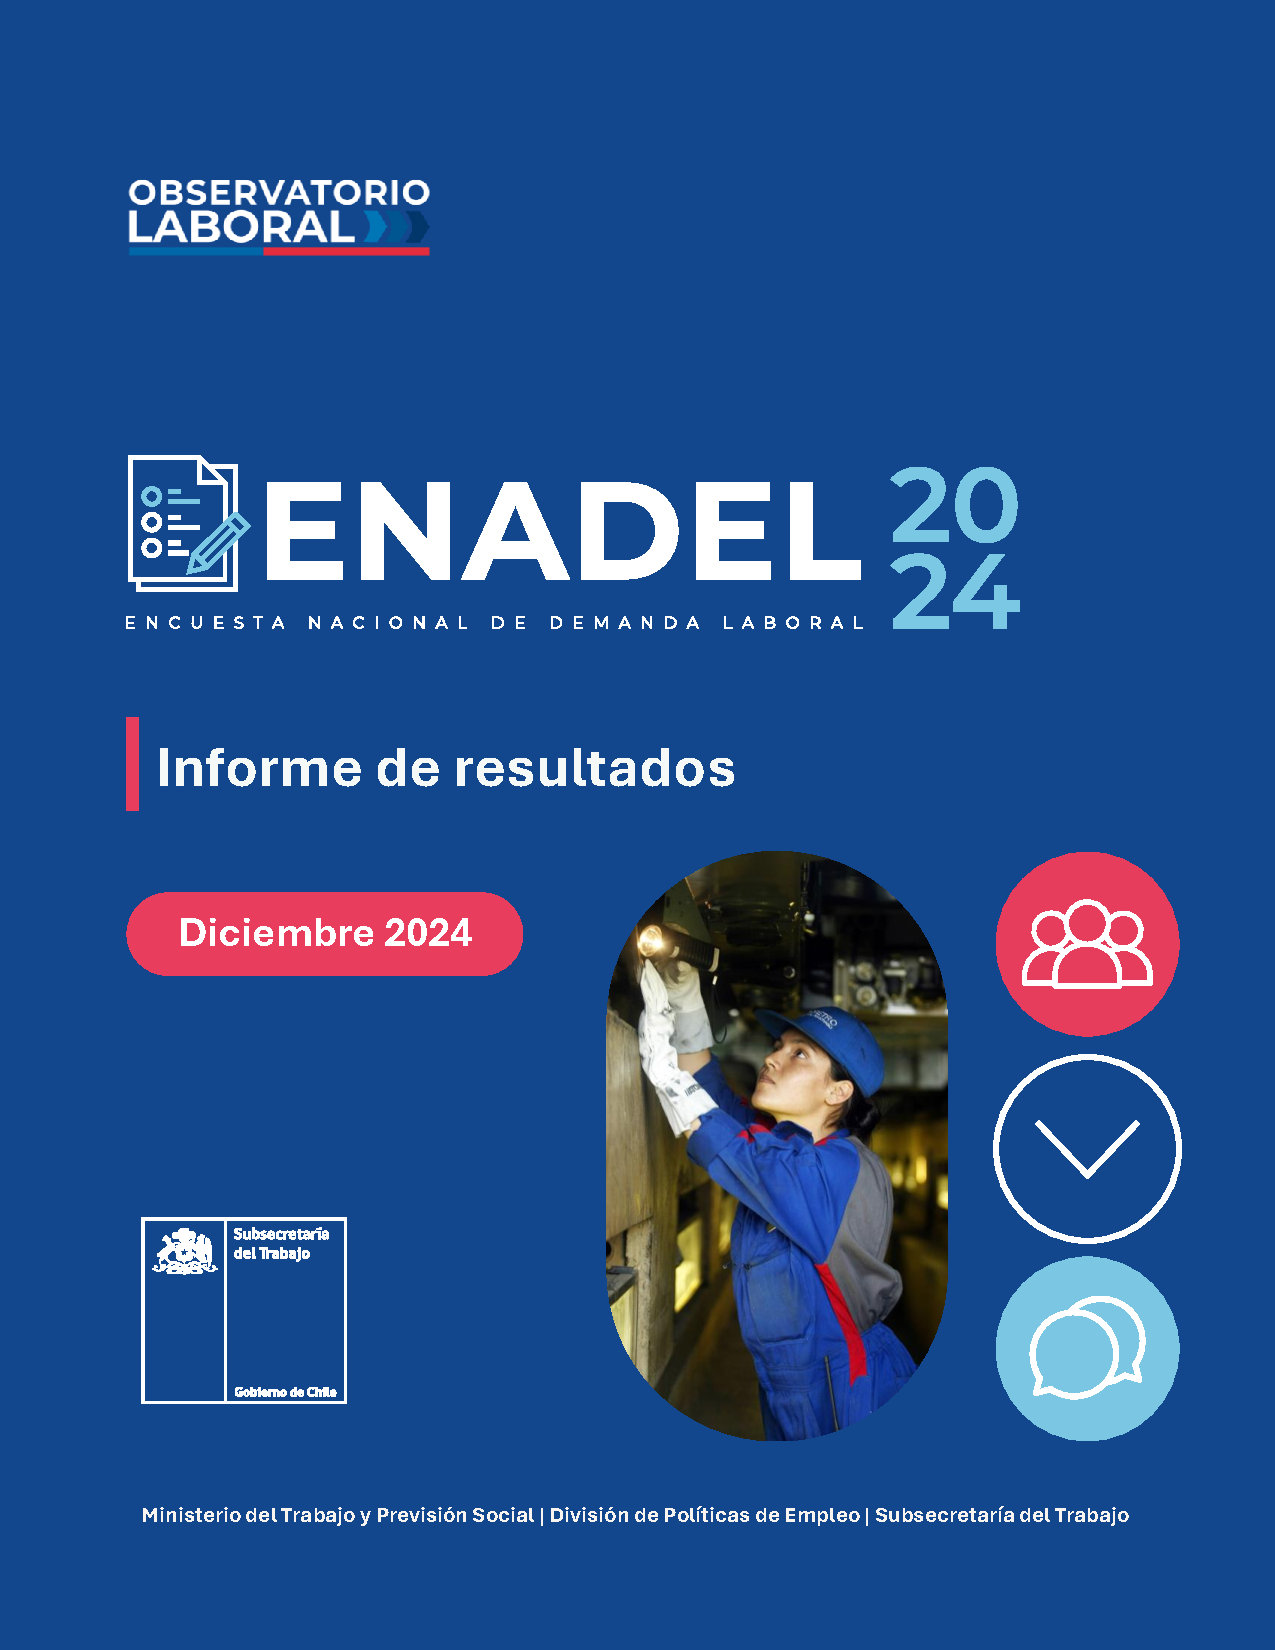
\includepdf[pages=-]{../Quarto/Portada/Portada_ENADEL 2024.pdf}


\definecolor{customblue}{HTML}{12468d}

\pagecolor{customblue} 
\thispagestyle{empty} 
\color{white}

\centering


\includegraphics[width=0.5\textwidth]{../Logotipo ENADEL/Logotipo ENADEL-02.png}
\vspace{2cm}

\noindent Ministerio del Trabajo y Previsión Social

Departamento de intermediación y prospección laboral\textbackslash{}
Subsecretaría del Trabajo

\justifying

El presente documento analiza los resultados de la Encuesta Nacional de
Demanda Laboral (ENADEL) 2024, que busca identificar y caracterizar el
capital humano requerido por las empresas de los distintos sectores
productivos del país, generando información sobre la demanda actual de
ocupaciones de las empresas, detectando requisitos y problemas de
contratación. A diferencia de las versiones anteriores de esta encuesta,
la actual versión abarca 15 sectores de actividad económica, ayuda a
identificar prioridades de capacitación y se añade el foco sobre el
impacto que está teniendo la incorporación de nuevas tecnologías y los
eventos climáticos extremos sobre los trabajadores.

\newpage
\nopagecolor
\color{black}
\renewcommand{\contentsname}{Índice} 
\tableofcontents

\newpage

La Encuesta Nacional de Demanda Laboral (ENADEL) 2024, desarrollada por
el Departamento de intermediación y prospección laboral de La
Subsecretaría del Trabajo, tiene como propósito principal identificar y
caracterizar las necesidades de capital humano en distintos sectores
productivos. La ENADEL 2024 analiza aspectos clave como las ocupaciones
de difícil cobertura, las brechas de competencias y habilidades, así
como los efectos de fenómenos disruptivos, como la incorporación de
nuevas tecnologías y eventos climáticos extremos, sobre la demanda
laboral. Además, esta encuesta permite profundizar en los requisitos y
problemas de contratación, abordando las prioridades de capacitación y
formación laboral en el país. Este informe, por tanto, busca ofrecer una
visión integral de las tendencias y retos del mercado laboral chileno,
proporcionando información clave para la formulación de políticas
públicas efectivas y el fortalecimiento del capital humano.

\section{Capítulo I: Contexto y caracterización de
empresas}\label{capuxedtulo-i-contexto-y-caracterizaciuxf3n-de-empresas}

El primer capítulo se centra en contextualizar y caracterizar a las
empresas participantes de la Encuesta Nacional de Demanda Laboral
(ENADEL) 2024. En este apartado se busca comprender la estructura y
distribución de las empresas a nivel nacional, diferenciando por tipo de
propiedad, tamaño, región y sector productivo. Con respecto a estos
sectores de actividad económica, se profundiza con respecto a los
sectores de Agricultura, ganadería, silvicultura y pesca, Industrias
manufactureras,Suministro de electricidad, gas, vapor y aire
acondicionado, Suministro de agua; evacuación de aguas residuales,
gestión de desechos y descontaminación, Construcción,
Comercio,Transporte y almacenamiento, Actividades de alojamiento y de
servicio de comidas, Información y comunicaciones, Actividades
financieras y de seguros, Actividades inmobiliarias, Actividades
profesionales, científicas y técnicas, Actividades de servicios
administrativos y de apoyo, Actividades artísticas, de entretenimiento y
recreativas y Otras actividades de servicios.

Asimismo, se examinan características relevantes de las empresas que
configuran la base del mercado laboral actual, con el fin de establecer
un panorama detallado sobre la composición y dinámica de los sectores
productivos. Este análisis otorga un marco inicial para interpretar la
demanda laboral en los siguientes capítulos, destacando patrones y
diferencias que permiten identificar regiones y sectores de mayor
demanda laboral así como los desafíos futuros asociados a la generación
de empleo en el país.

\FloatBarrier

\newpage

\subsection{Regiones y ubicación de
sucursales}\label{regiones-y-ubicaciuxf3n-de-sucursales}

La muestra de ENADEL 2024 encuesta a 4.816 empresas que suman 330.937
trabajadores (a nivel muestral). Estas representan a 245.339 empresas y
17.358.952 trabajadores a nivel nacional.

La Tabla~\ref{tbl-region} muestra la distribución en las distintas
regiones del país, dónde la Macrozona norte\footnote{La macrozona norte
  corresponde a las regiones de Arica y Parinacota, Tarapacá,
  Antofagasta y Atacama. La macrozona centro incluye las regiones de
  Coquimbo y Valparaíso. La macrozona centro-sur abarca las regiones de
  O'Higgins, Maule, Ñuble y Biobío. La macrozona sur comprende las
  regiones de La Araucanía, Los Ríos y Los Lagos. Finalmente, la
  macrozona austral corresponde a las regiones de Aysén y Magallanes.}
representa un total de \text{14,5}\% de las empresas del país y un
\text{6,8}\% del total de trabajadores. En la Macrozona centro se ubican
el \text{15}\% de las empresas y el \text{14,5}\% de los trabajadores.
Un \text{7,3}\% de las empresas y un \text{6,1}\% de los trabajadores se
encuentran en la región Metropolitana. La Macrozonza Centro Sur
contempla el \text{30,5}\% de las empresas y al \text{29,8}\% de
trabajadores del país. Por su parte, un \text{24,7}\% de las empresas
del país se encuentran en la Macrozona Sur, la que comprende al
\text{40,6}\% de los trabajadores a nivel nacional.

Por último, en la Macrozona Austral se encuentran el \text{7,9}\% de las
empresas y el \text{2,2}\% de los trabajadores de Chile.

\vspace{5mm}

\FloatBarrier

\begin{table}

\caption{\label{tbl-region}Resultados de la encuesta}

\centering{

\centering
\begin{tabular}{>{\raggedright\arraybackslash}p{6cm}>{\raggedright\arraybackslash}p{3cm}>{\raggedright\arraybackslash}p{3cm}}
\toprule
Región & \% Empresas & \% Trabajadores\\
\midrule
Arica y Parinacota & 3,3\% & 1\%\\
Tarapacá & 3,9\% & 1\%\\
Antofagasta & 2,2\% & 0,8\%\\
Atacama & 5,1\% & 4\%\\
Coquimbo & 7,3\% & 9,3\%\\
\addlinespace
Valparaíso & 7,7\% & 5,2\%\\
Metropolitana & 7,3\% & 6,1\%\\
O'Higgins & 9,2\% & 7,8\%\\
Maule & 9,8\% & 7,5\%\\
Ñuble & 9,9\% & 14,3\%\\
\addlinespace
Biobío & 1,6\% & 0,2\%\\
La Araucanía & 2,7\% & 4,6\%\\
Los Ríos & 14,4\% & 32\%\\
Los Lagos & 7,6\% & 4\%\\
Aysén & 3,5\% & 0,8\%\\
\addlinespace
Magallanes & 4,4\% & 1,4\%\\
\bottomrule
\multicolumn{3}{l}{\rule{0pt}{1em}Fuente: Elaboración propia utilizando datos de ENADEL 2024.}\\
\end{tabular}

}

\end{table}%

\newpage

La Figura~\ref{fig-mapa} ilustra la cantidad de empresas por región, las
regiones con más cantidad de empresas corresponden a Los Ríos, Ñuble y
Maule con un total de 4.851, 3.340 y 3.279 empresas respectivamente. Por
su parte, las regiones de Araucanía, Antofagasta y Biobío registran la
menor cantidad de empresas, con 910 o menos organizaciones.

\begin{figure}[H]

\caption{\label{fig-mapa}Empresas por región}

\centering{

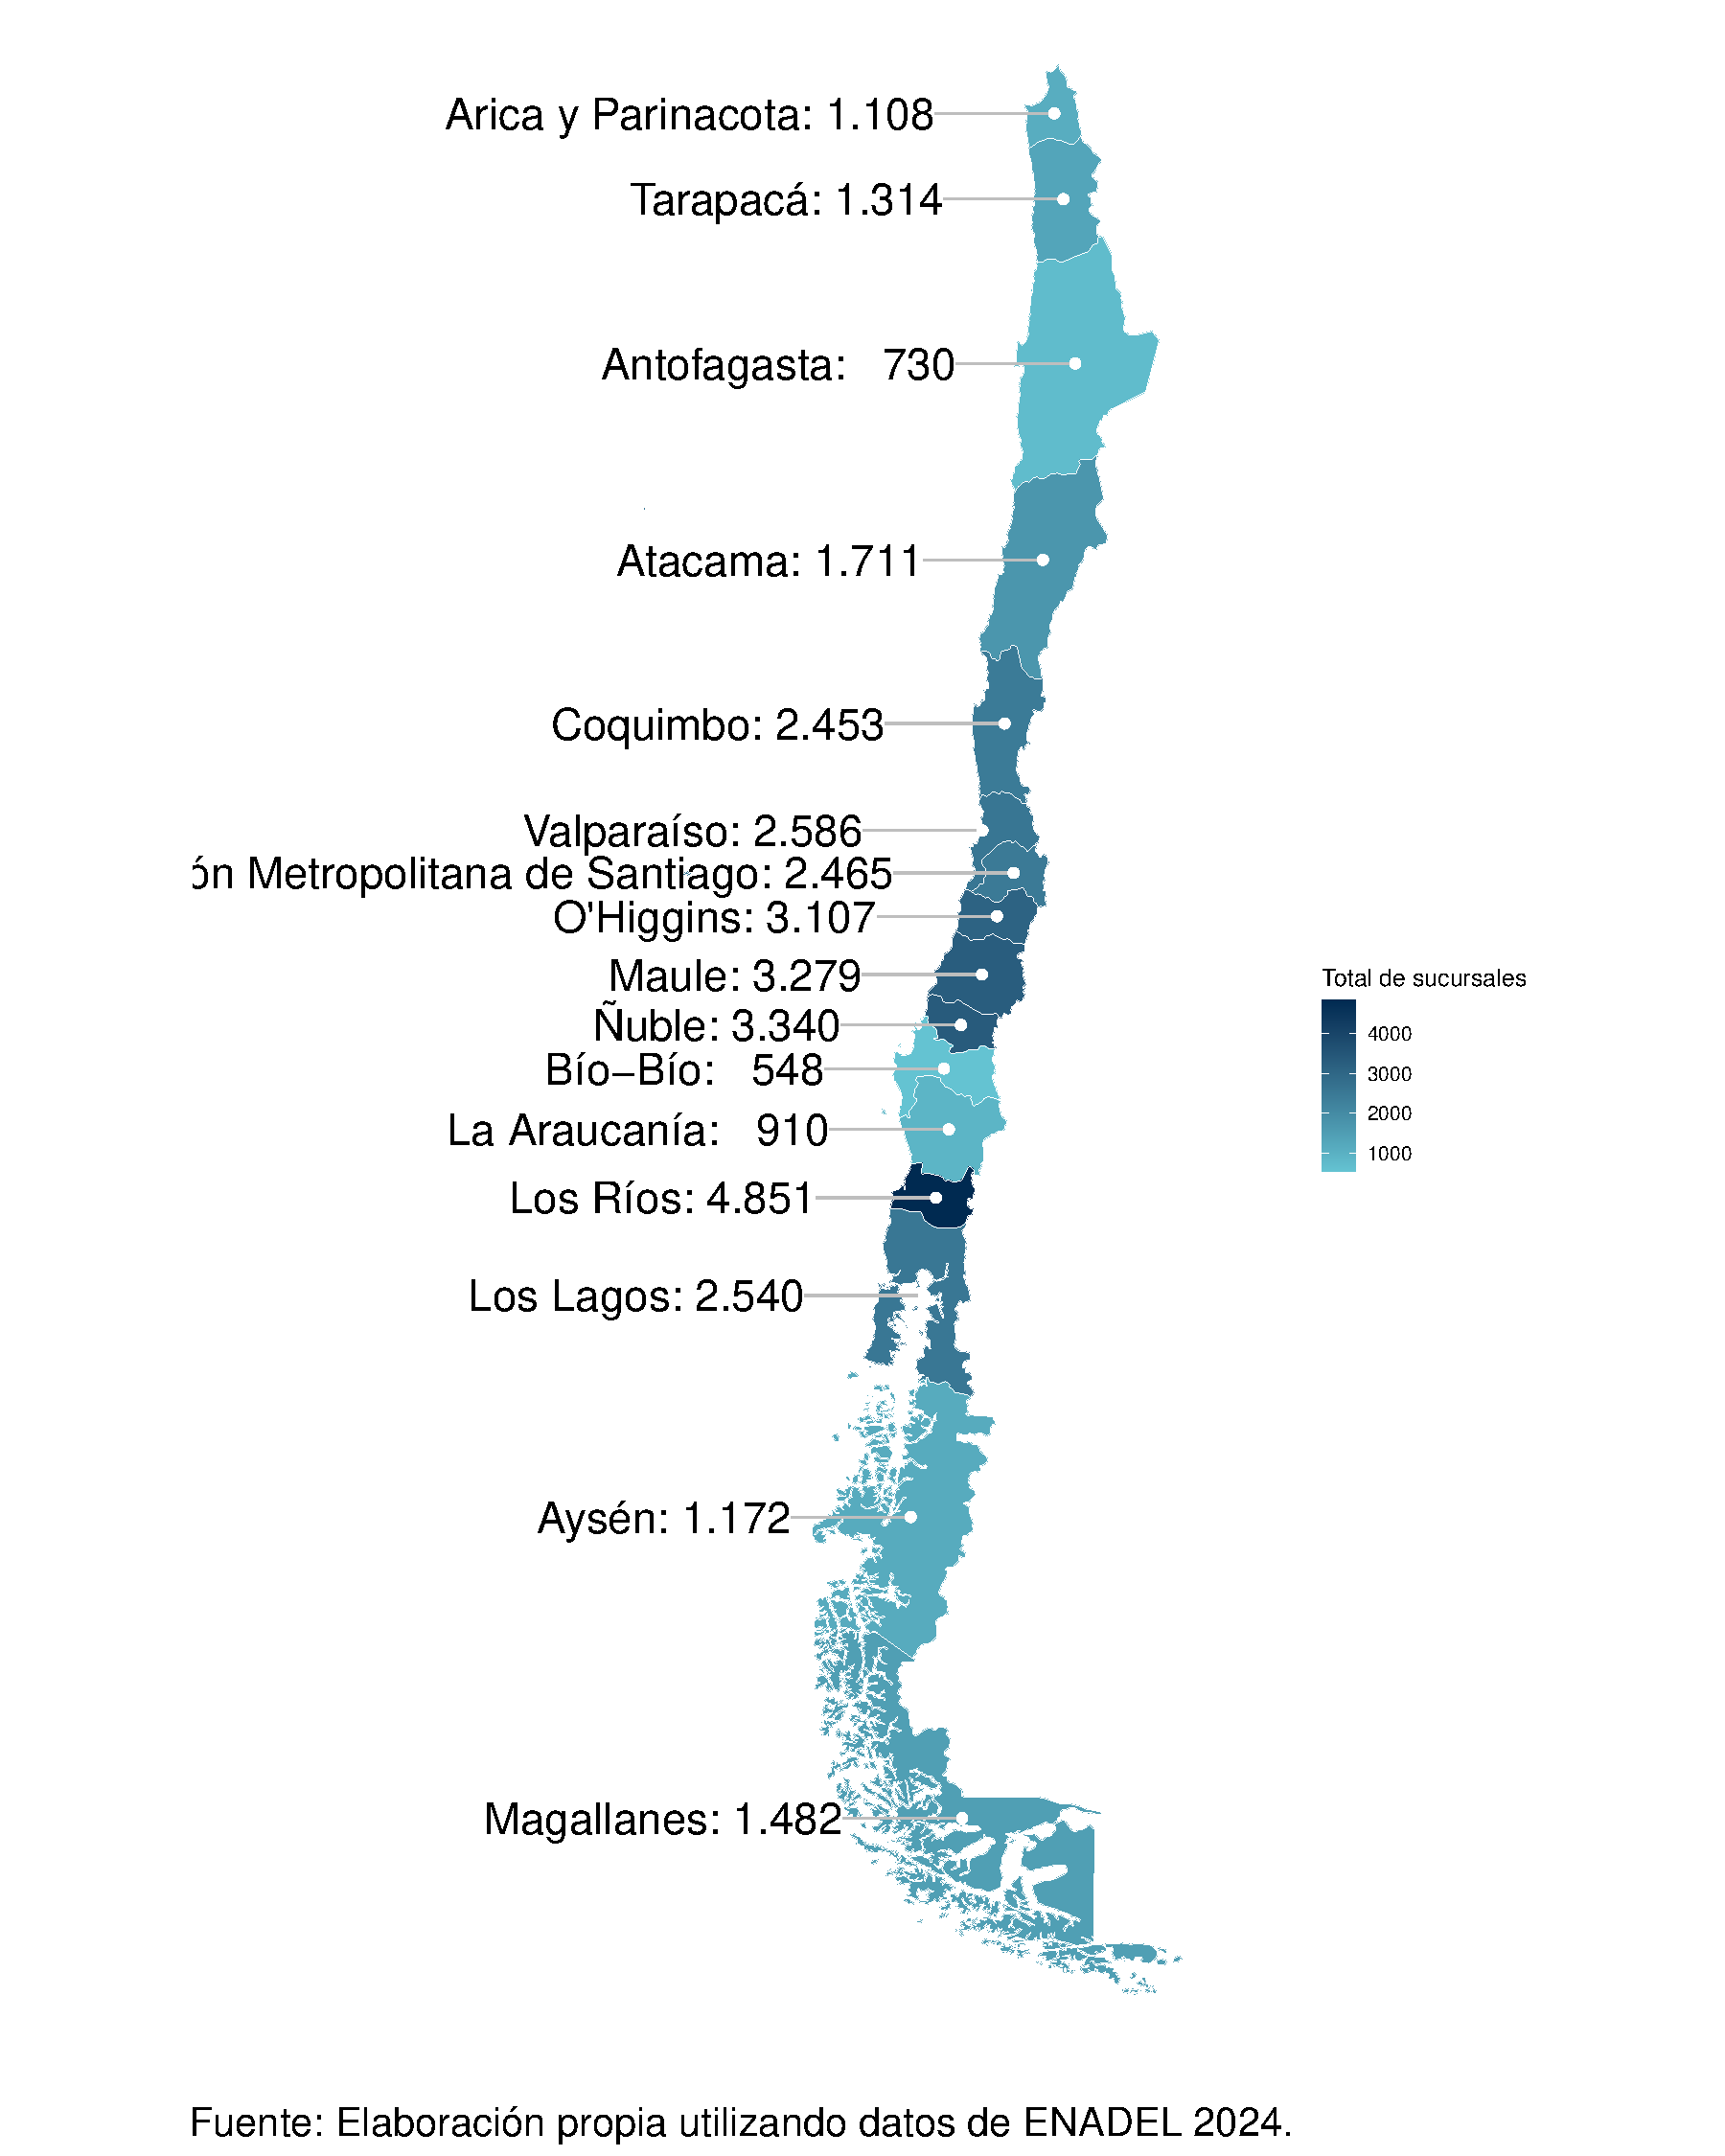
\includegraphics{reporte_2024_files/figure-pdf/fig-mapa-1.pdf}

}

\end{figure}%

\newpage

La Figura~\ref{fig-burbujas} ilustra la cantidad de empresas que tienen
sucursales en más de una región. La región con más sucursales (sedes no
principales) corresponde a 4 con un total de 13.110 que es equivalente
al 15,7\% del total de sucursales del país. En segundo lugar, la región
9 posee 8.739 filiales representando el 10,4\% del total de sucursales
del país. En la región 7 existen 8.236 sucursales. Demanera contraria,
las regiones donde las empresas tienen menor cantidad de filiales
corresponden a 6 ( 2.158), 5 ( 2.081) y 2 ( 1.907).

\FloatBarrier

\begin{figure}[H]

\caption{\label{fig-burbujas}Sucursales por región}

\centering{

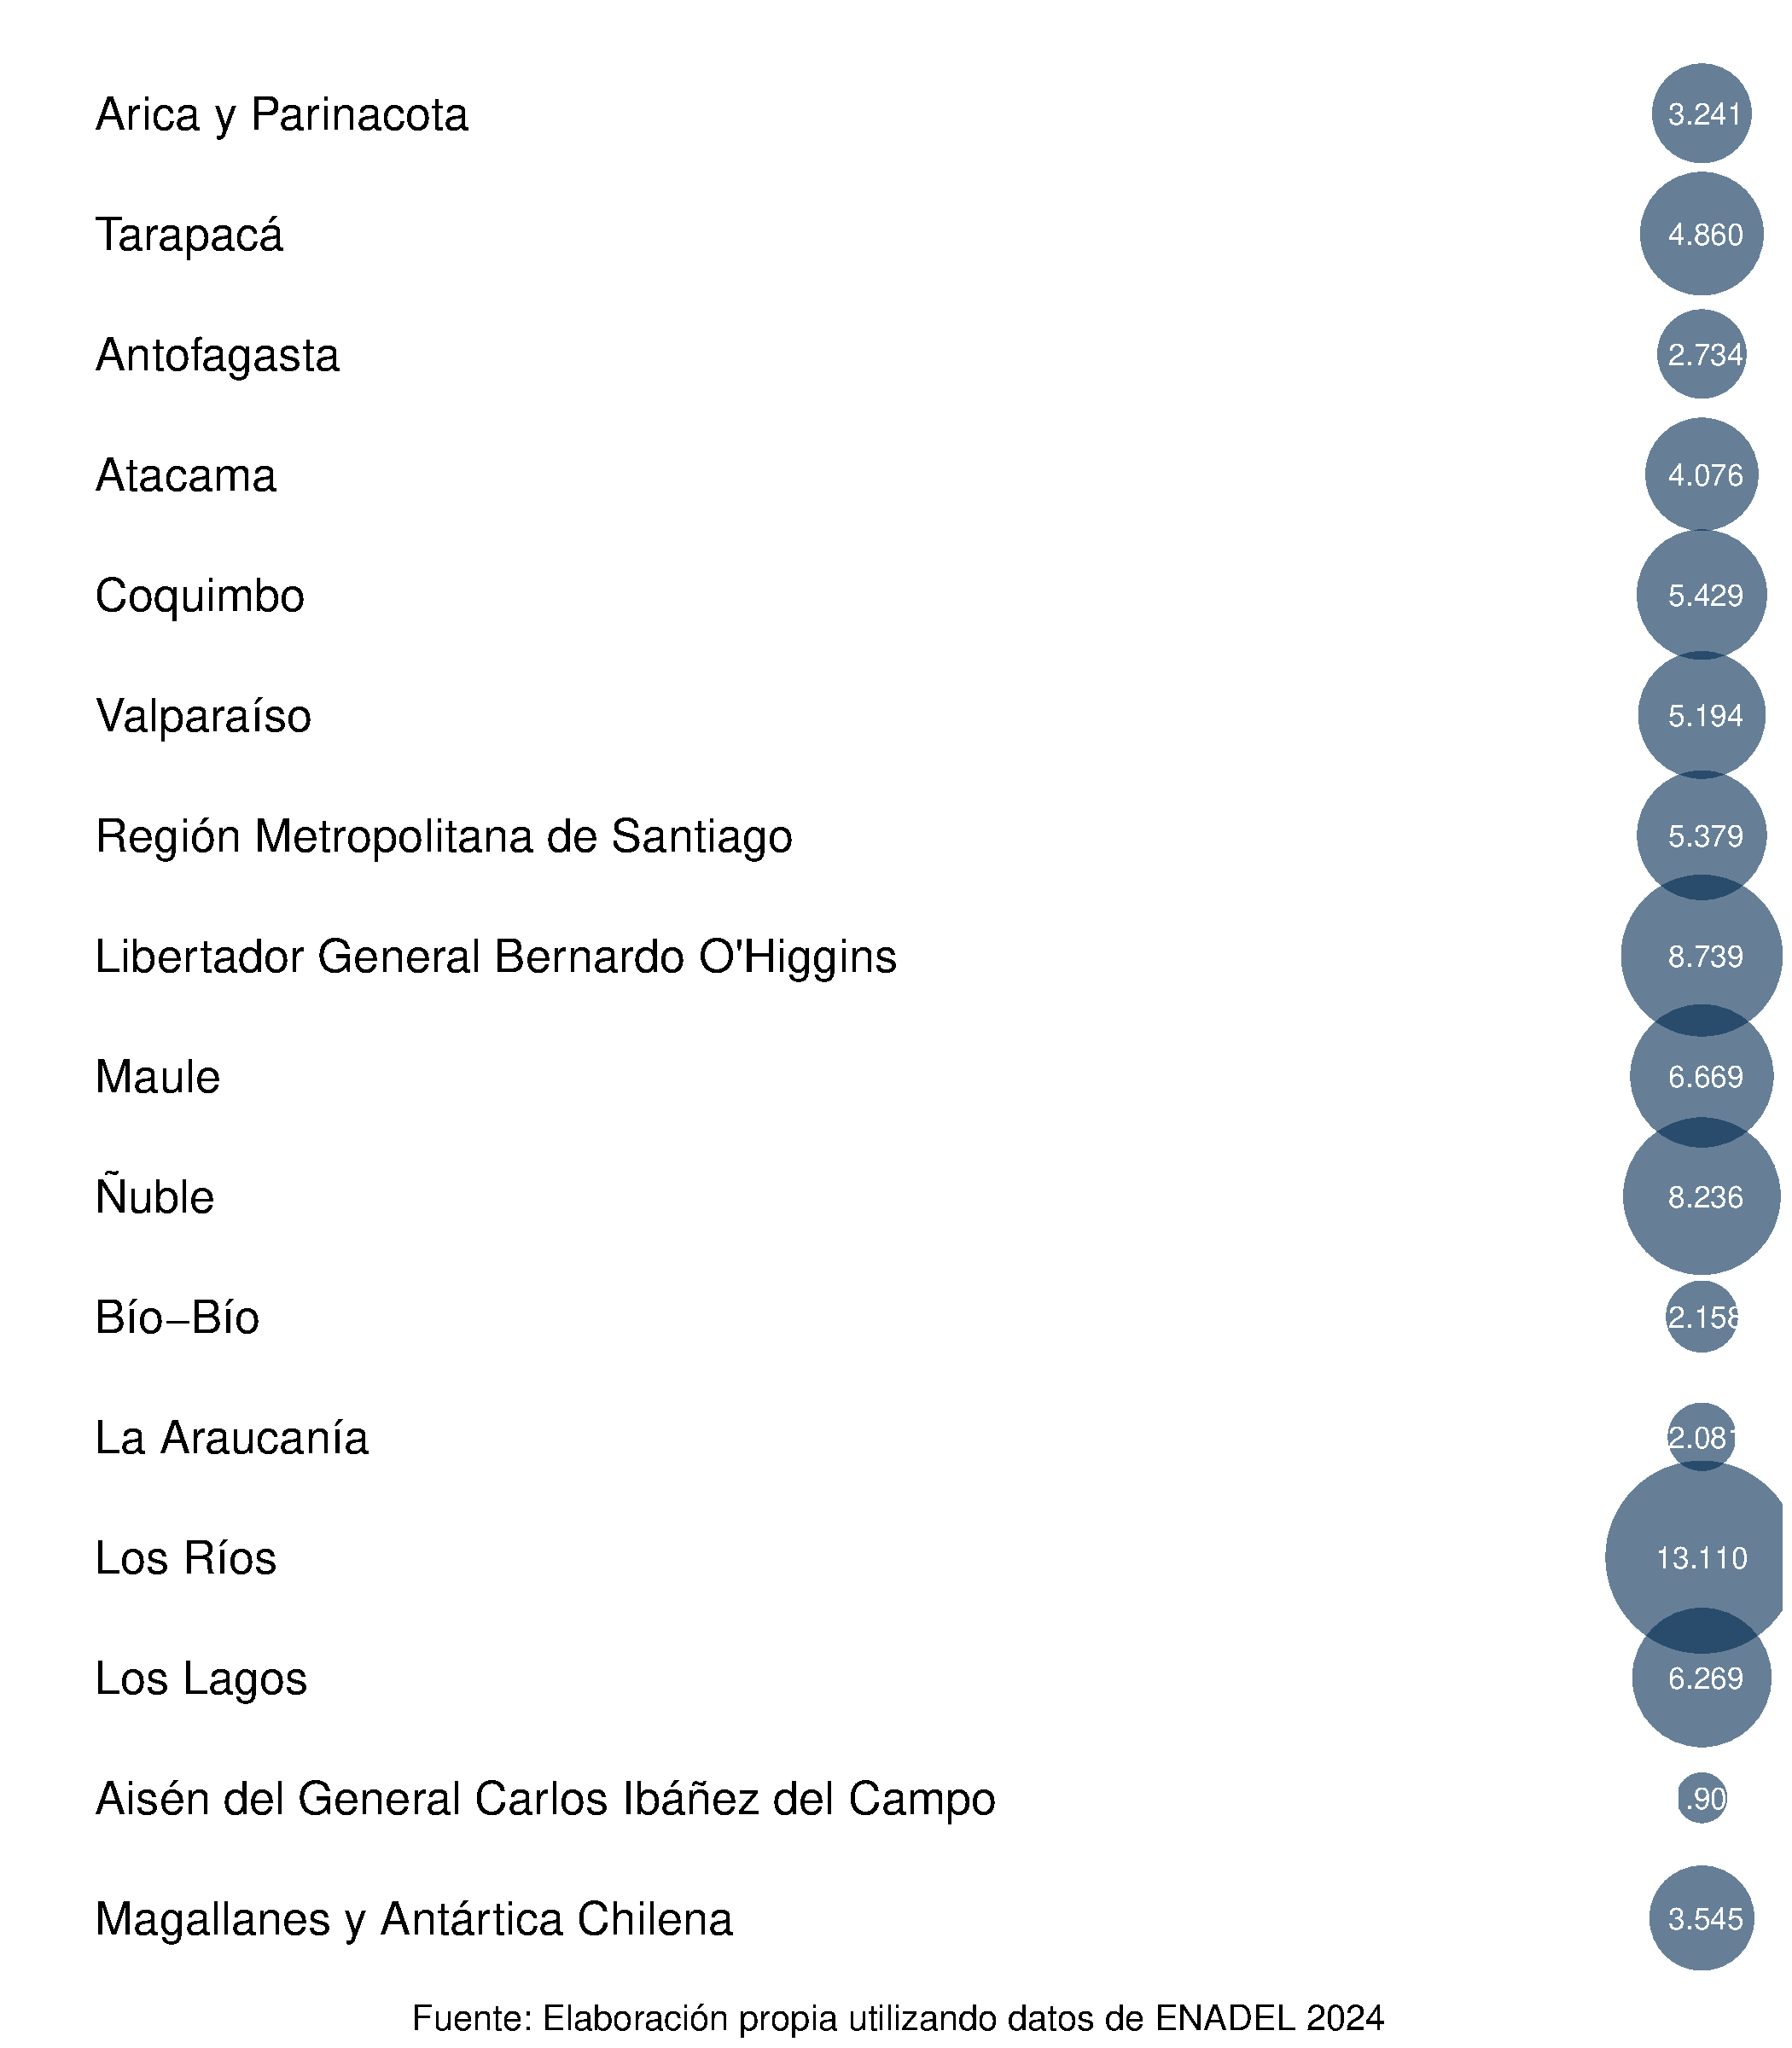
\includegraphics{reporte_2024_files/figure-pdf/fig-burbujas-1.pdf}

}

\end{figure}%

\FloatBarrier

\subsection{Tamaño de empresas}\label{tamauxf1o-de-empresas}

La Figura~\ref{fig-tam} muestra como se distribuyen las empresas por
tamaño de empresa, indicando los porcentajes acorde al tamaño de las
empresas según su número de trabajadores. Según el g´rafico, el
\text{81,8}\% de las empresas tiene menos de 50 trabajadores -que
representa el \text{20,8}\% de los trabajadores-. Un \text{12,8}\% de
las empresas son medianas de tamaño (entre 50 y 199 trabajadores),
dentro de estas organizaciones se encuentra el \text{17}\% de los
trabajadores del país. Y un \text{5,4}\% de las empresas corresponde a
empresas grandes con 200 trabajadores o más, lo que equivale al
\text{62,2}\% del total de trabajadores.

\FloatBarrier

\begin{figure}[H]

\caption{\label{fig-tam}Distribución tamaño de empresas según número de
trabajadores}

\centering{

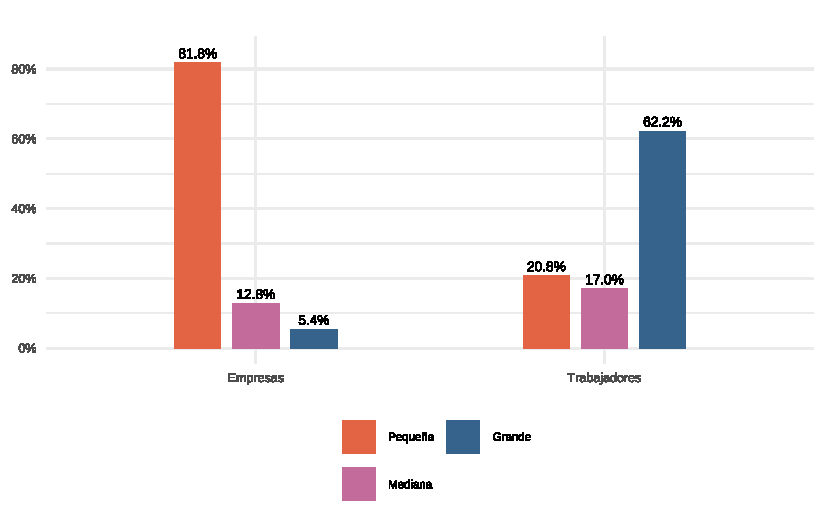
\includegraphics[width=1\textwidth,height=\textheight]{reporte_2024_files/figure-pdf/fig-tam-1.pdf}

}

\end{figure}%

\FloatBarrier

En la Figura~\ref{fig-tamvent} se aprecia la distribución de las
empresas por tamaño según el volumen de venta declarado por las
empresas. El gráfico muestra que un \text{14,5}\% de las empresas tienen
un volumen de venta menores a 2.400 UF (microempresa), el \text{39,8}\%
posee un volumen de venta anual entre 2.400 y 24.999 UF (``Pequeñas'') y
el \text{22}\% venden entre 25.000 y 100.000 UF al año (``Mediana'').
Sin embargo, el \text{49}\% de los trabajadores están en empresas
grandes (más de 100.000 UF).

\begin{figure}[H]

\caption{\label{fig-tamvent}Distribución empresas según tamaño de
ventas}

\centering{

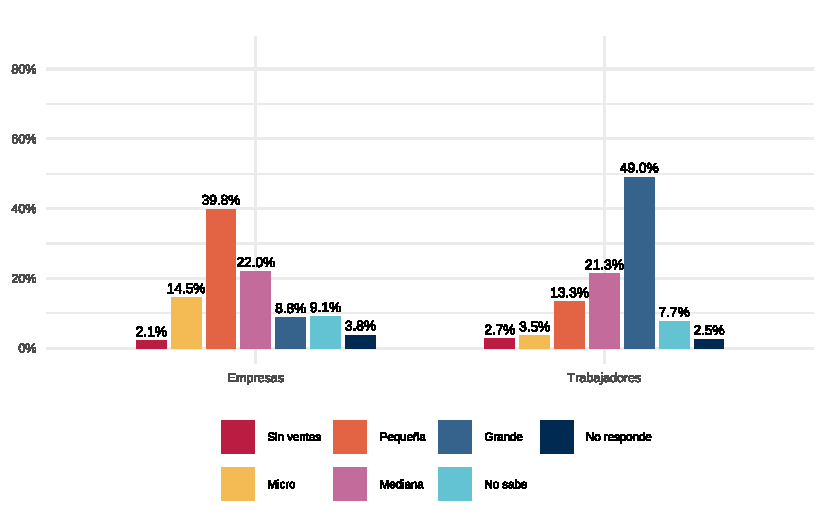
\includegraphics[width=1\textwidth,height=\textheight]{reporte_2024_files/figure-pdf/fig-tamvent-1.pdf}

}

\end{figure}%

Al revisar la distribución por sector de actividad económica
Tabla~\ref{tbl-acteco} se tiene que el sector de Construcción
(\text{19}\%) , seguido por el sector Transporte y almacenamiento
(\text{14,3}\%) y el sector de Minería (\text{11,1}\%) concentran la
mayor cantidad de empresas a nivel nacional. Con respecto al volumen de
trabajadores, el sector Actividades profesionales y técnicas lidera
(\text{17,7}\%) seguido por el sector Suministro de agua y gestión de
desechos (\text{15,4}\%) y el sector de Agricultura, silvicultura y
pesca que, siendo sector intensivo en trabajo, un \text{9}\% de las
empresas acumula el \text{14,4} de trabajadores y trabajadoras.

\FloatBarrier

\begin{table}

\caption{\label{tbl-acteco}Empresas y trabajadores según sector de
actividad económica}

\centering{

\centering
\begin{tabular}{>{\raggedright\arraybackslash}p{9cm}ll}
\toprule
Actividad Económica & \% Empresas & \% Trabajadores\\
\midrule
Actividades profesionales y técnicas & 8,3\% & 17,7\%\\
Suministro de agua y gestión de  desechos & 9,9\% & 15,4\%\\
Agricultura, silvicultura y pesca & 9\% & 14,4\%\\
Construcción & 19\% & 14,2\%\\
Minería & 11,1\% & 11,4\%\\
\addlinespace
Comercio & 9,4\% & 8,6\%\\
Transporte y almacenamiento & 14,3\% & 5\%\\
Actividades inmobiliarias & 4,9\% & 3,6\%\\
Suministro de electricidad y gas & 2,3\% & 2,8\%\\
Servicios administrativos y de apoyo & 2,8\% & 2,1\%\\
\addlinespace
Alojamiento y de servicio de comida & 3,6\% & 1,8\%\\
Actividades financieras y de seguros & 3,2\% & 1,7\%\\
Industrias manufactureras & 1,1\% & 0,7\%\\
Información y comunicaciones & 1,2\% & 0,7\%\\
\bottomrule
\multicolumn{3}{l}{\rule{0pt}{1em}Fuente: Elaboración propia utilizando datos de ENADEL 2024.}\\
\end{tabular}

}

\end{table}%

\FloatBarrier

\subsection{Estructura corporativa}\label{estructura-corporativa}

En este subapartado se analiza la distribución de las empresas a nivel
nacional según sus características de estructura corporativa. En primer
lugar, se examina el tipo de propiedad de las empresas, diferenciando
entre privadas (nacionales o extranjeras), estatales y mixtas.
Posteriormente, se estudia la distribución de las empresas que prestan
servicios bajo la figura de subcontratación, considerando tanto el
sector de actividad económica como la región. Finalmente, se describe la
distribución de las organizaciones según su pertenencia a conglomerados
y gremios empresariales.

La Tabla~\ref{tbl-tipo_propiedad} muestra la distribución de las
empresas según su tipo de propiedad. Se presentan los datos en términos
de tamaño muestral de empresas, cantidad de empresas expandidas a nivel
poblacional, número de trabajadores en la muestra y trabajadores
representados a nivel poblacional. La gran mayoría de las organizaciones
corresponden al tipo de propiedad Privada nacional, que representa el
\text{97}\% de las empresas y concentra el \text{85,1}\% de los
trabajadores del país. En contraste, otros tipos de propiedad tienen una
representación significativamente menor. Por ejemplo, sólo el
\text{1,7}\% corresponde a empresas del tipo de propiedad Privada
extranjera, lo que equivale a un total del \text{9,7}\% de los
trabajadores del país. A su vez, el \text{0,4}\% corresponde a empresas
del tipo de propiedad Estatal, lo que equivale al \text{2,1}\% de los
trabajadores. Y un \text{0,9}\% corresponde a empresas del tipo de
propiedad Mixta, conteniendo el \text{9,7}\% de los trabajadores del
país.

\begin{table}

\caption{\label{tbl-tipo_propiedad}Tipo de propiedad de empresas}

\centering{

\centering
\begin{tabular}{>{\raggedright\arraybackslash}p{3cm}>{\raggedright\arraybackslash}p{2.5cm}>{\raggedright\arraybackslash}p{2.5cm}>{\raggedright\arraybackslash}p{2.5cm}>{\raggedright\arraybackslash}p{2.5cm}}
\toprule
Tipo de propiedad & Empresas (Muestra) & Empresas Estimadas & Trabajadores (Muestra) & Trabajadores Estimados\\
\midrule
Privada nacional & 4.677 & 238.074 & 277.885 & 14.776.364\\
Privada extranjera & 78 & 4.064 & 36.729 & 1.682.395\\
Estatal & 21 & 1.005 & 6.528 & 357.124\\
Mixta & 40 & 2.195 & 9.795 & 543.070\\
Total & 4.816 & 245.338 & 330.937 & 17.358.953\\
\bottomrule
\multicolumn{5}{l}{\rule{0pt}{1em}Fuente: Elaboración propia utilizando datos de ENADEL 2024.}\\
\end{tabular}

}

\end{table}%

En la Figura~\ref{fig-subcontratos_sector} se aprecia la distribución de
empresas que prestan servicios a otras empresas a través del
subcontrato\footnote{La subcontratación se entiende como el trabajo
  realizado para un empleador denominado contratista o subcontratista,
  quien ejecuta obras o servicios por cuenta y riesgo propio para una
  empresa principal, dueña de la obra o faena.} según sector de
actividad económica. Los sectores de actividad económica con mayor
presencia de empresas que prestan servicios de subcontrato son los
sectores de Construcción (\text{17,9}\%), Transporte y almacenamiento
(\text{16,7}\%) y Servicios administrativos y de apoyo (\text{13,4}\%)
respectivamente. Los sectores que tienen menor presencia de empresas que
prestan servicios de subcontratación son los sectores de Actividades
inmobiliarias (\text{1,3}\%), Suministro de electricidad y gas
(\text{1,1}\%) y Actividades financieras y de seguros (\text{0,6}\%).

\begin{figure}[H]

\caption{\label{fig-subcontratos_sector}Gráfico subcontrato según sector
de actividad económica}

\centering{

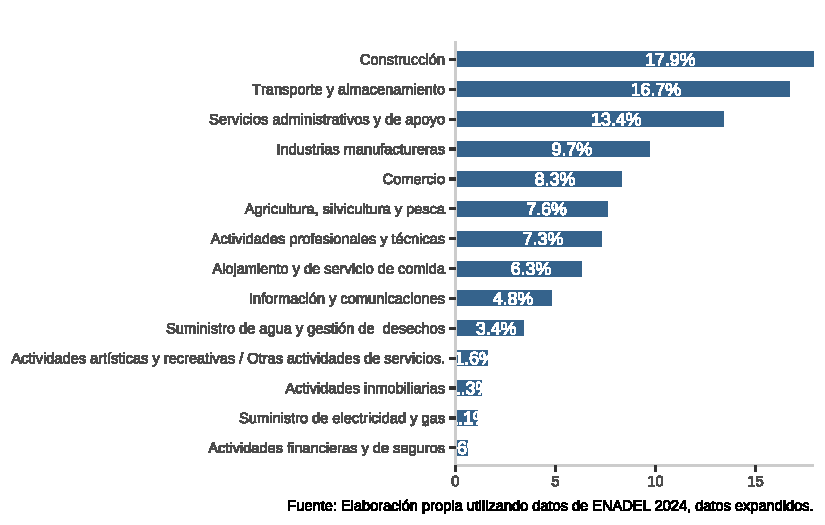
\includegraphics[width=1\textwidth,height=\textheight]{reporte_2024_files/figure-pdf/fig-subcontratos_sector-1.pdf}

}

\end{figure}%

La Tabla~\ref{tbl-subcontratos_region} indica la distribución de las
empresas que prestan servicios bajo la figura del subcontrato según
región de ubicación de la empresa, la región de Biobío es la que posee
la mayor parte (\text{14,2}\%) de empresas subcontratistas del país.
Seguida por la región, del Los Lagos la que concentra el \text{9}\% de
empresas subcontratistas. En tercer lugar, la región de La Araucanía
posee el \text{8,7}\% de este tipo de relación contractual.

\begin{table}

\caption{\label{tbl-subcontratos_region}Distribución regional de
Empresas que operan mediante Subcontratación}

\centering{

\centering
\begin{tabular}{>{\raggedright\arraybackslash}p{9cm}>{\raggedright\arraybackslash}p{3cm}}
\toprule
Región & \% Empresas en subcontrato\\
\midrule
Arica y Parinacota & 3,6\%\\
Tarapacá & 3,4\%\\
Antofagasta & 5,2\%\\
Atacama & 5,2\%\\
Coquimbo & 4,7\%\\
\addlinespace
Valparaíso & 6,7\%\\
Metropolitana & 6,7\%\\
O'Higgins & 5,4\%\\
Maule & 8,1\%\\
Ñuble & 7,2\%\\
\addlinespace
Biobío & 14,2\%\\
La Araucanía & 8,7\%\\
Los Ríos & 7\%\\
Los Lagos & 9\%\\
Aysén & 2,3\%\\
\addlinespace
Magallanes & 2,9\%\\
\bottomrule
\multicolumn{2}{l}{\rule{0pt}{1em}Fuente: Elaboración propia utilizando datos de ENADEL 2024.}\\
\end{tabular}

}

\end{table}%

La Tabla~\ref{tbl-conglomerado_gremio} presenta los porcentajes de las
empresas que pertencen a conglomerados y gremios\footnote{Un
  conglomerado es un grupo de empresas dedicadas a negocios no
  necesariamente relacionados, pero que tienen un controlador o
  accionista mayoritario común o que se encuentra relacionado mediante
  pactos o sociedades. Estos conglomerados ejercen control sobre las
  empresas afiliadas mediante estructuras piramidales, series
  accionarias preferentes y tenencias cruzadas de acciones (La Porta et
  al., 1999; Wolfenzon, 1999; Bebchuck, Kraakman y Triantis, 1999). En
  Chile, según el Decreto Ley 2757, los gremios empresariales
  corresponden a un tipo de asociación voluntaria de empresas que
  pertenecen a un mismo sector económico o industria, con el propósito
  de representar y defender intereses comunes}. Se aprecia que los
sectores de Comercio con Transporte y almacenamiento y Agricultura,
silvicultura y pesca poseen los mayores niveles de empresas
conglomeradas con el \text{14,7}\%, \text{11,7}\% y \text{11,6}\% de
empresas correspondientes.

Con respecto al poder asociativo de las empresas, el \text{15,6}\% de
las empresas del sector Comercio pertenecen a un gremio empresarial. De
igual forma, el sector Alojamiento y de servicio de comida presenta un
\text{15,6}\% de empresas asociadas, mientras que el sector
\text{15,6}\% cuenta con un Construcción de empresas pertenecientes a
algún gremio empresarial.

\FloatBarrier

\begin{table}

\caption{\label{tbl-conglomerado_gremio}Empresas pertenecientes a
Conglomerados y Gremios}

\centering{

\centering
\begin{tabular}{>{\raggedright\arraybackslash}p{11cm}ll}
\toprule
Actividad Económica & \% Conglomerados & \% Gremios\\
\midrule
Comercio & 14,7\% & 15,6\%\\
Transporte y almacenamiento & 11,7\% & 10\%\\
Agricultura, silvicultura y pesca & 11,6\% & 10,1\%\\
Industrias manufactureras & 11,2\% & 11\%\\
Construcción & 10,7\% & 14,5\%\\
\addlinespace
Servicios administrativos y de apoyo & 9,5\% & 4,6\%\\
Alojamiento y de servicio de comida & 6,8\% & 15,6\%\\
Actividades inmobiliarias & 5,5\% & 3,9\%\\
Actividades profesionales y técnicas & 3,7\% & 4,2\%\\
Actividades artísticas y recreativas / Otras actividades de servicios. & 3,7\% & 1,7\%\\
\addlinespace
Actividades financieras y de seguros & 3,7\% & 1,4\%\\
Información y comunicaciones & 3,3\% & 4,5\%\\
Suministro de agua y gestión de  desechos & 2\% & 1,8\%\\
Suministro de electricidad y gas & 1,8\% & 1\%\\
\bottomrule
\multicolumn{3}{l}{\rule{0pt}{1em}Fuente: Elaboración propia utilizando datos de ENADEL 2024.}\\
\end{tabular}

}

\end{table}%

\FloatBarrier

\newpage

\section{Capítulo II: Demanda Laboral y Ocupaciones de Difícil
Cobertura}\label{capuxedtulo-ii-demanda-laboral-y-ocupaciones-de-difuxedcil-cobertura}

A continuación, se identifica y caracteriza la demanda laboral de las
empresas durante 2024. En primer lugar, se presentan las cifras
relativas a la dotación actual de personal en las empresas, seguido de
un análisis de las salidas y contrataciones realizadas para determinar
la demanda de trabajo de las organizaciones, incluyendo los principales
perfiles ocupacionales contratados, sus competencias y los requisitos
asociados.En segundo lugar, se presentan las vacantes
actuales\footnote{Número de ofertas de trabajo que se esperan abrir en
  lo que queda del año 2024.} y futuras\footnote{Número de ofertas de
  trabajo que se esperan abrir durante el año 2025.}. Para finalizar el
análisis se identifican las principales ocupaciones de difícil cobertura
presentando las dificultades más relevantes que enfrentan estas
posiciones no cubiertas.

\subsection{Dotación}\label{dotaciuxf3n}

En cuanto a la dotación actual de las empresas, la
Tabla~\ref{tbl-dotacion_resumen} indica que la cantidad actual de
personas empleadas asciende a un total de 17.358.952 a nivel nacional.
Además, se aprecia que la mayor parte de la dotación de trabajadores se
encuentra en la categoría de Contrato Indefinido con un total de
11.776.473 trabajadores, de los cuales el 32,7\% corresponden a mujeres
y un 67,2\% a personal masculino. Si bien la distribución según sexo del
trabajador se mantiene en el resto de categorías contractuales, es la
categoría de Honorario donde hay mayor presencia de mujeres
trabajadoras, lo que da cuenta de que las mujeres se encuentran en una
condición de independencia y flexibilidad, pero al mismo tiempo de mayor
inestabilidad y ausencia de protección laboral.

\FloatBarrier

\begin{table}

\caption{\label{tbl-dotacion_resumen}Dotación actual de las empresas
segpun tipo de relación contractual}

\centering{

\centering
\begin{tabular}{>{\raggedright\arraybackslash}p{3cm}lllll}
\toprule
Categoría & Total & Mujer & Hombre & \% Mujer & \% Hombre\\
\midrule
Indefinido & 11.776.473 & 3.852.312 & 7.915.540 & 32,7\% & 67,2\%\\
Plazo fijo & 5.056.494 & 1.656.658 & 3.399.548 & 32,8\% & 67,2\%\\
Honorario & 302.955 & 137.111 & 165.803 & 45,3\% & 54,7\%\\
Dotación total & 17.358.952 & 5.713.742 & 11.645.210 & 32,9\% & 67,1\%\\
\bottomrule
\multicolumn{6}{l}{\rule{0pt}{1em}Fuente: Elaboración propia utilizando datos de ENADEL 2024.}\\
\end{tabular}

}

\end{table}%

\FloatBarrier

\subsection{Contrataciones últimos 12
meses}\label{contrataciones-uxfaltimos-12-meses}

La Tabla~\ref{tbl-contratados_u12} sólo muestra aquellas ocupaciones
para las cuáles el coeficiente de variación es menor a 50\%\footnote{La
  convención es considerar cómo robustas estimaciones con un cv menor al
  15\%. Dado que estas son pocas, se presentan todas las ocupaciones con
  un cv menor a 50\%.}. Las ocupaciones más contratadas en los últimos
12 meses fueron ``Auxiliares de aseo de oficinas, hoteles y otros
establecimientos'' con 222.241 contrataciones, en segundo lugar con
171.388 contrataciones, ``Obreros de explotaciones agrícolas'' y
``Empleados encargados del control de abastecimiento e inventario'' con
141.683 contrataciones. \FloatBarrier

\begin{table}

\caption{\label{tbl-contratados_u12}Contratados últimos 12 meses, por
ocupación.}

\centering{

\centering
\begin{tabular}{r>{\raggedright\arraybackslash}p{10cm}ll}
\toprule
CIUO\_08 & Glosa & Contratados & cv\\
\midrule
9112 & Auxiliares de aseo de oficinas, hoteles y otros establecimientos & 222.241 & 31,4\%\\
9211 & Obreros de explotaciones agrícolas & 171.388 & 36,6\%\\
4321 & Empleados encargados del control de abastecimiento e inventario & 141.683 & 34,3\%\\
5414 & Guardias de seguridad & 124.867 & 48,5\%\\
3123 & Supervisores de la construcción & 86.389 & 29,9\%\\
\addlinespace
3113 & Técnicos en electricidad & 85.976 & 37\%\\
2142 & Ingenieros civiles, ingenieros en construcción y constructores civiles & 79.051 & 34,3\%\\
9313 & Obreros de la construcción de edificios & 70.138 & 36,8\%\\
4110 & Trabajadores de tareas administrativas generales & 54.087 & 49,2\%\\
9412 & Ayudantes de cocina & 51.284 & 32,1\%\\
\addlinespace
7112 & Albañiles & 46.799 & 45\%\\
\bottomrule
\multicolumn{4}{l}{\rule{0pt}{1em}Fuente: Elaboración propia utilizando datos de ENADEL 2024.}\\
\end{tabular}

}

\end{table}%

\FloatBarrier

La Tabla~\ref{tbl-contratados_sector} muestra la comparativa entre los
sectores de actividad económica con respecto a la cantidad de puestos de
trabajos contratados los últimos 12 meses, el sector de Agricultura,
silvicultura y pesca con 3.047.175 contrataciones. En segundo lugar, el
sector de Servicios administrativos y de apoyo contrató un total de
1.197.570 personas, seguido del sector de Construcción con un total de
498.805 ocupaciones contratadas durante los últimos 12 meses. Dentro de
los sectores que menos vacantes contratados tuvieron fueron los sectores
de Actividades inmobiliarias con 27.375 puestos de trabajo, el sector
Actividades financieras y de seguros con 16.032 vacantes contratadas y
el sector Suministro de electricidad y gas con 10.017 vacantes
contratadas durante el último año.

\FloatBarrier

\begin{table}

\caption{\label{tbl-contratados_sector}Contratados últimos 12 meses por
sector de actividad económica.}

\centering{

\centering
\begin{tabular}{>{\raggedright\arraybackslash}p{9cm}l}
\toprule
Glosa & Contratados\\
\midrule
Agricultura, silvicultura y pesca & 3.047.175\\
Servicios administrativos y de apoyo & 1.197.570\\
Construcción & 498.805\\
Industrias manufactureras & 449.081\\
Comercio & 356.693\\
\addlinespace
Transporte y almacenamiento & 253.568\\
Alojamiento y de servicio de comida & 118.735\\
Actividades profesionales y técnicas & 86.084\\
Suministro de agua y gestión de  desechos & 44.339\\
Actividades artísticas y recreativas / Otras actividades de servicios. & 37.359\\
\addlinespace
Información y comunicaciones & 27.481\\
Actividades inmobiliarias & 27.375\\
Actividades financieras y de seguros & 16.032\\
Suministro de electricidad y gas & 10.017\\
\bottomrule
\multicolumn{2}{l}{\rule{0pt}{1em}Fuente: Elaboración propia utilizando datos de ENADEL 2024.}\\
\end{tabular}

}

\end{table}%

Respecto del nivel educacional de los contratados, la
Tabla~\ref{tbl-contratados_u12_educ} presenta la cantidad de cargos
contratados los últimos doce meses\footnote{Desde 2023 al 31 de mayo de
  2024} y su nivel educacional. Se observa que la mayoría de los puestos
de trabajo contratados el último año no exigen algún requisito con
respecto al nivel educacional, específicamente, existieron 2.291.164
contrataciones cuyo nivel educacional fue Sin requisito. En segundo
lugar, se observan 2.040.096 personas contratadas con nivel de Educación
básica. También se indica que existieron 1.705.901 contrataciones donde
los trabajadores contaban con un nivel educacional de Educación media
científico humanista.

\begin{table}

\caption{\label{tbl-contratados_u12_educ}Nivel educacional de
ocupaciones contratadas los últimos doce meses}

\centering{

\centering
\begin{tabular}{>{\raggedright\arraybackslash}p{9cm}ll}
\toprule
Nivel educacional & Contratados & cv\\
\midrule
Sin requisito & 2.291.164 & 16,3\%\\
Educación básica & 2.040.096 & 70,2\%\\
Educación media científico humanista & 1.705.901 & 28,8\%\\
Educación media técnico profesional & 196.494 & 16,3\%\\
Profesional (universitaria) & 99.572 & 34,4\%\\
\addlinespace
Técnico superior & 81.336 & 11,5\%\\
Profesional con postgrado & 3.242 & 70,7\%\\
\bottomrule
\multicolumn{3}{l}{\rule{0pt}{1em}Fuente: Elaboración propia utilizando datos de ENADEL 2024.}\\
\end{tabular}

}

\end{table}%

La Tabla~\ref{tbl-certificaciones_tot} abarca las certificaciones,
licencias o requisitos exigidos de los principales cargos/ocupaciones
que las empresas contrataron durante los últimos doce meses (durante
2023 al 31 de mayo de 2024). La certificación más solicitada corresponde
a Certificados de Antecedentes la que fue requisito en 40.934 cargos
contratados los últimos 12 meses. La segunda certificación más exigida
fue Certificado de Experiencia Laboral en 5.986 cargos y Certificado de
Estudios fue la tercera certificación más exigida con un total de 1.377
cargos contratados los últimos 12 meses. Por el contrario,
Capacitaciones relacionadas al rubro y ocupación fue la certificación
menos requerida, con 77 contrataciones donde fue necesaria dicha
certificación.

\begin{table}

\caption{\label{tbl-certificaciones_tot}Certificaciones de ocupaciones
contratadas los últimos doce meses}

\centering{

\centering
\begin{tabular}{>{\raggedright\arraybackslash}p{9cm}ll}
\toprule
Certificación/Licencia requeridos & Contratados & cv\\
\midrule
Certificados de Antecedentes & 40.934 & 3,7\%\\
Certificado de Experiencia Laboral & 5.986 & 10,1\%\\
Certificado de Estudios & 1.377 & 21\%\\
Licencia de conducir Clase A & 829 & 30,7\%\\
Licencia de conducir Clase B & 591 & 35,8\%\\
\addlinespace
Certificados de acreditación de cursos & 230 & 48,3\%\\
Licencia de conducir Clase D & 146 & 61,8\%\\
Capacitaciones relacionadas al rubro y ocupación & 77 & 100\%\\
\bottomrule
\multicolumn{3}{l}{\rule{0pt}{1em}Fuente: Elaboración propia utilizando datos de ENADEL 2024.}\\
\end{tabular}

}

\end{table}%

Al profundizar, qué ocupaciones poseen mayor dotación al interior de
cada sector de actividad económica, la
Figura~\ref{fig-dotacion_sector_ocupacion} ilustra cuáles son las
ocupaciones con mayor cantidad de trabajadores según cada sector. En la
figura se aprecia que dentro del sector Comercio, la ocupación con mayor
cantidad de puestos de trabajo (Número total de personas empleadas a
tiempo completo o parcial) corresponde a Empleados encargados del
control de abastecimiento e inventario con un total de 119.105. Dentro
del sector Industrias manufactureras, la ocupacióin de Obreros de
explotaciones agrícolas cuenta con la mayor dotación de personal
(100.296). A su vez, en el sector Construcción existen un total de
61.176 trabajadores en la ocupación Empleados encargados del control de
abastecimiento e inventario.

Por otro lado, los sectores con menos dotación de personal fueron
Suministro de electricidad y gas, cuya ocupación con mayor dotación de
trabajadores ( 5.166) fue Auxiliares y ayudantes de servicios
estadísticos, financieros y de seguros, seguido del sector Actividades
inmobiliarias con 5.050 trabajadores en la ocupación de Auxiliares de
aseo de oficinas, hoteles y otros establecimientos. Finalmente, en el
sector de Actividades financieras y de seguros la ocupación con mayor
cantidad de personas trabajando corresponde a Ingenieros en prevención
de riesgos y otros profesionales de la seguridad e higiene laboral y
ambiental, cuya cantidad de trabajadores fue de 768.

\begin{figure}[H]

\caption{\label{fig-dotacion_sector_ocupacion}Oficios con mayor cantidad
de trabajadores por sector}

\centering{

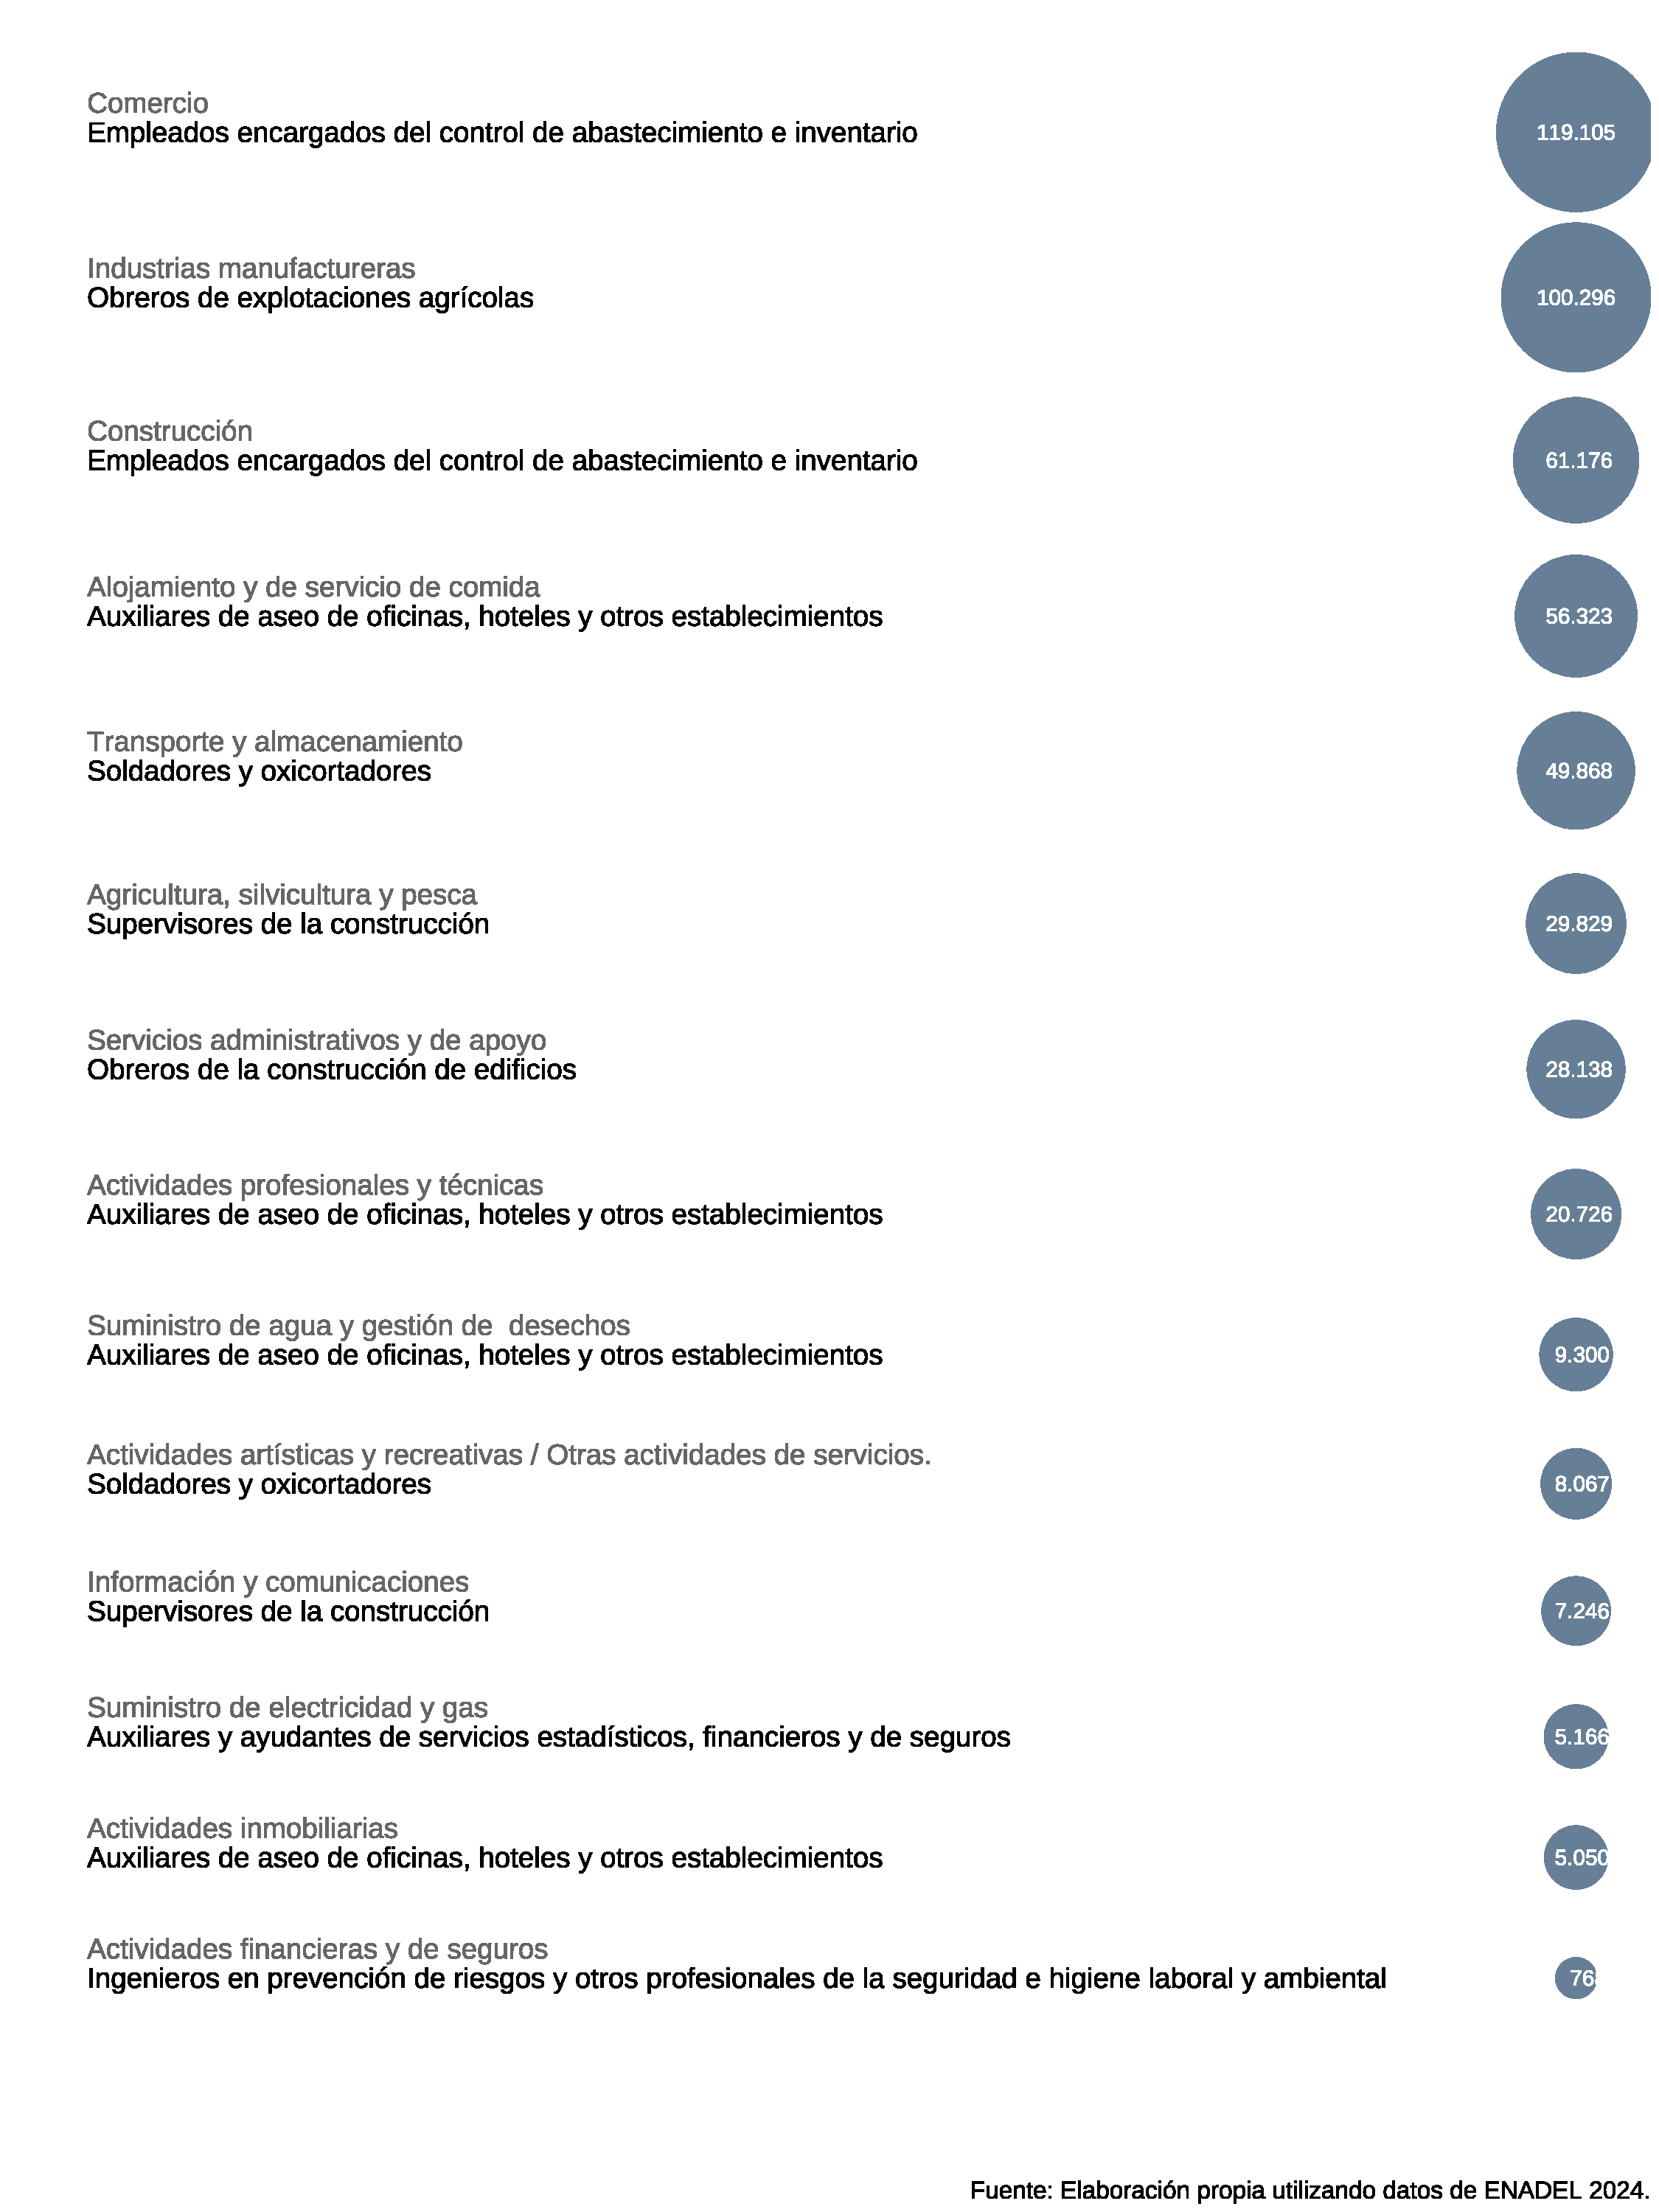
\includegraphics[width=1\textwidth,height=\textheight]{reporte_2024_files/figure-pdf/fig-dotacion_sector_ocupacion-1.pdf}

}

\end{figure}%

Con respecto al tipo de relación contractual entre las empresas y sus
trabajadores, la Tabla~\ref{tbl-dotacion_indefinido} presenta las
ocupaciones con mayor dotación dentro de cada sector económico para las
cuáles el coeficiente de variación es menor a 50\%\footnote{La
  convención es considerar cómo robustas estimaciones con un cv menor al
  15\%. Dado que estas son pocas, se presentan todas las ocupaciones con
  un coeficiente de variación menor a 50\%.} cuya relación contractual
corresponde a un contrato indefinido. En el sector Comercio, se
encuentran 83.148 trabajadores desempeñándose en la ocupación de
Empleados encargados del control de abastecimiento e inventario. Dentro
del sector Industrias manufactureras, existen 79.843 trabajadores
desempeñándose en la ocupación de Ingenieros en prevención de riesgos y
otros profesionales de la seguridad e higiene laboral y ambiental.
Mientras que en el sector Alojamiento y de servicio de comida la
ocupación con mayor cantidad de personal es Ingenieros en prevención de
riesgos y otros profesionales de la seguridad e higiene laboral y
ambiental con un total de 38.613 trabajadores.

\begin{table}

\caption{\label{tbl-dotacion_indefinido}Dotación contrato indefinido por
sector de actividad económica}

\centering{

\centering
\begin{tabular}{>{\raggedright\arraybackslash}p{5cm}>{\raggedright\arraybackslash}p{7cm}>{\raggedright\arraybackslash}p{2cm}>{\raggedright\arraybackslash}p{2cm}}
\toprule
Sector de actividad económica & Glosa & Contratados & CV\\
\midrule
Comercio & Empleados encargados del control de abastecimiento e inventario & 83.148 & 43,1\%\\
Industrias manufactureras & Ingenieros en prevención de riesgos y otros profesionales de la seguridad e higiene laboral y ambiental & 79.843 & 47\%\\
Alojamiento y de servicio de comida & Auxiliares de aseo de oficinas, hoteles y otros establecimientos & 38.613 & 40\%\\
Construcción & Empleados encargados del control de abastecimiento e inventario & 37.432 & 36,3\%\\
Transporte y almacenamiento & Soldadores y oxicortadores & 30.552 & 44,3\%\\
\addlinespace
Agricultura, silvicultura y pesca & Vendedores y asistentes de venta de tiendas, almacenes y puestos de mercado & 22.893 & 43,8\%\\
Servicios administrativos y de apoyo & Obreros de la construcción de edificios & 20.071 & 32,2\%\\
Actividades profesionales y técnicas & Auxiliares de aseo de oficinas, hoteles y otros establecimientos & 12.183 & 32,6\%\\
Suministro de agua y gestión de  desechos & Auxiliares de aseo de oficinas, hoteles y otros establecimientos & 7.556 & 42,2\%\\
Información y comunicaciones & Soldadores y oxicortadores & 6.051 & 49,5\%\\
\addlinespace
Actividades artísticas y recreativas / Otras actividades de servicios. & Soldadores y oxicortadores & 5.676 & 45,8\%\\
Suministro de electricidad y gas & Auxiliares y ayudantes de servicios estadísticos, financieros y de seguros & 5.166 & 0\%\\
Actividades inmobiliarias & Auxiliares de aseo de oficinas, hoteles y otros establecimientos & 5.041 & 40,4\%\\
Actividades financieras y de seguros & Ingenieros en prevención de riesgos y otros profesionales de la seguridad e higiene laboral y ambiental & 651 & 0\%\\
\bottomrule
\multicolumn{4}{l}{\rule{0pt}{1em}Fuente: Elaboración propia utilizando datos de ENADEL 2024.}\\
\end{tabular}

}

\end{table}%

En cuanto a los trabajadores que se desempeñan bajo contrato de plazo
fijo Tabla~\ref{tbl-dotacion_plazofijo} presenta las ocupaciones con
mayor dotación dentro de cada sector económico para las cuáles el
coeficiente de variación es menor a 50\%. En el sector Agricultura,
silvicultura y pesca, se encuentran 28.309 trabajadores desempeñándose
en la ocupación de Auxiliares de aseo de oficinas, hoteles y otros
establecimientos. Dentro del sector Construcción, existen 21.518
trabajadores desempeñándose en la ocupación de Auxiliares de aseo de
oficinas, hoteles y otros establecimientos. Mientras que en el sector
Transporte y almacenamiento la ocupación con mayor cantidad de personal
es Auxiliares de aseo de oficinas, hoteles y otros establecimientos con
un total de 8.070 trabajadores.

\begin{table}

\caption{\label{tbl-dotacion_plazofijo}Dotación contrato a plazo fijo
por sector de actividad económica}

\centering{

\centering
\begin{tabular}{>{\raggedright\arraybackslash}p{5cm}>{\raggedright\arraybackslash}p{7cm}>{\raggedright\arraybackslash}p{2cm}>{\raggedright\arraybackslash}p{2cm}}
\toprule
Sector de actividad económica & Glosa & Plazo Fijo & CV\\
\midrule
Agricultura, silvicultura y pesca & Auxiliares de aseo de oficinas, hoteles y otros establecimientos & 28.309 & 45,7\%\\
Construcción & Auxiliares de aseo de oficinas, hoteles y otros establecimientos & 21.518 & 37,4\%\\
Transporte y almacenamiento & Auxiliares de aseo de oficinas, hoteles y otros establecimientos & 8.070 & 43,9\%\\
Alojamiento y de servicio de comida & Obreros de explotaciones agrícolas & 6.904 & 42,8\%\\
Actividades profesionales y técnicas & Auxiliares de aseo de oficinas, hoteles y otros establecimientos & 5.462 & 40,4\%\\
\addlinespace
Comercio & Secretarios administrativos y ejecutivos & 4.437 & 42,7\%\\
Industrias manufactureras & Supervisores de la construcción & 4.174 & 37,9\%\\
Servicios administrativos y de apoyo & Albañiles & 1.505 & 46\%\\
Actividades financieras y de seguros & Ingenieros en prevención de riesgos y otros profesionales de la seguridad e higiene laboral y ambiental & 117 & 0\%\\
\bottomrule
\multicolumn{4}{l}{\rule{0pt}{1em}Fuente: Elaboración propia utilizando datos de ENADEL 2024.}\\
\end{tabular}

}

\end{table}%

La Tabla~\ref{tbl-dotacion_honorarios} presenta las ocupaciones con
mayor dotación dentro de cada sector económico, correspondientes a
trabajadores a honorarios (coeficiente de variación es menor a 50\%). En
el sector Alojamiento y de servicio de comida, la ocupación con más
trabajadores bajo esta modalidad contractual corresponde a Auxiliares de
aseo de oficinas, hoteles y otros establecimientos con un total de 3.544
trabajadores. Dentro del sector Industrias manufactureras, existen 1.823
trabajadores desempeñándose en la ocupación de Auxiliares de aseo de
oficinas, hoteles y otros establecimientos. Por otro lado, la ocupación
con mayor cantidad de personal en el sector Construcción es Auxiliares
de aseo de oficinas, hoteles y otros establecimientos con un total de
1.027 trabajadores.

\begin{table}

\caption{\label{tbl-dotacion_honorarios}Dotación trabajadores a
honorarios por sector de actividad económica}

\centering{

\centering
\begin{tabular}{>{\raggedright\arraybackslash}p{5cm}>{\raggedright\arraybackslash}p{7cm}>{\raggedright\arraybackslash}p{2cm}>{\raggedright\arraybackslash}p{2cm}}
\toprule
Sector de actividad económica & Glosa & Honorarios & CV\\
\midrule
Alojamiento y de servicio de comida & Auxiliares de aseo de oficinas, hoteles y otros establecimientos & 3.544 & 40,7\%\\
Industrias manufactureras & Auxiliares de aseo de oficinas, hoteles y otros establecimientos & 1.823 & 39,7\%\\
Construcción & Empleados encargados del control de abastecimiento e inventario & 1.027 & 43\%\\
Comercio & Guardias de seguridad & 1.021 & 41,9\%\\
Servicios administrativos y de apoyo & Empleados y asistentes de recursos humanos & 299 & 49,4\%\\
\addlinespace
Actividades financieras y de seguros & Obreros de carga & 58 & 0\%\\
\bottomrule
\multicolumn{4}{l}{\rule{0pt}{1em}Fuente: Elaboración propia utilizando datos de ENADEL 2024.}\\
\end{tabular}

}

\end{table}%

\subsection{Vacantes y Salidas}\label{vacantes-y-salidas}

La Figura~\ref{fig-vacantes} presenta las vacantes actuales\footnote{Número
  de ofertas de trabajo o vacantes abiertas al 31 de mayo del 2024.} y
las vacantes futuras, que corresponden a la cantidad estimada de puestos
de trabajo que se abrirán en los próximos doce meses. Este año, se
registraron 964.882 vacantes vacantes abiertas\footnote{Número de
  ofertas de trabajo o vacantes abiertas al 31 de mayo del 2024.} del
2024.. En cuanto a las vacantes futuras, estas se dividen en dos
categorías: los puestos de trabajo previstos para el resto del año 2024
(3.235.711) y las ofertas de empleo proyectadas para el año 2025
(4.620.639).

\FloatBarrier

\begin{figure}[H]

\caption{\label{fig-vacantes}Gráfico Vacantes}

\centering{

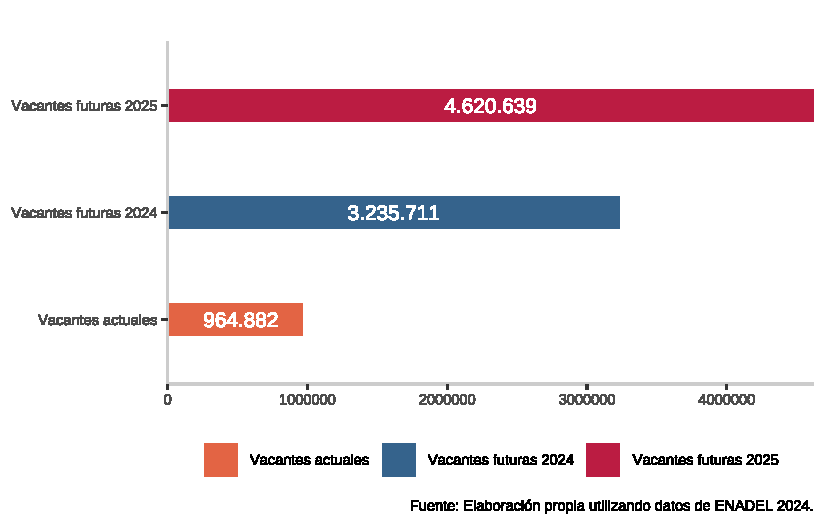
\includegraphics[width=1\textwidth,height=\textheight]{reporte_2024_files/figure-pdf/fig-vacantes-1.pdf}

}

\end{figure}%

En la Figura~\ref{fig-salidas_contrataciones} aparecen los porcentajes
correspondientes a las salidas (renuncias, despidos o ceses)\footnote{Renuncias
  y Ceses, terminaciones de empleados/as permanentes, de corto plazo o
  estacionales.} y contrataciones diferenciando por sexo de los
trabajadores. Durante los últimos 12 meses a nivel nacional hubo un
total de \text{1569395} renuncias, de las cuales el \text{34,7}\%
corresponde a renuncias hechas por mujeres, mientras que el
\text{64,5}\% de estas corresponden a renuncias hechas por hombres.

En cuanto a despidos (y ceses) \footnote{Ceses, terminaciones de
  empleados/as permanentes, de corto plazo o estacionales.}, en el
gráfico se observa que a nivel nacional existió un total de
\text{7040137}, de los cuales el \text{34,8}\% corresponde a casos de
despidos o terminaciones de empleos ocupados por mujeres, y un
\text{64,4}\% corresponde a despidos o ceses cuyos puestos de trabajos
eran ocupados por hombres.

\FloatBarrier

\begin{figure}[H]

\caption{\label{fig-salidas_contrataciones}Gráfico salidas y
contrataciones}

\centering{

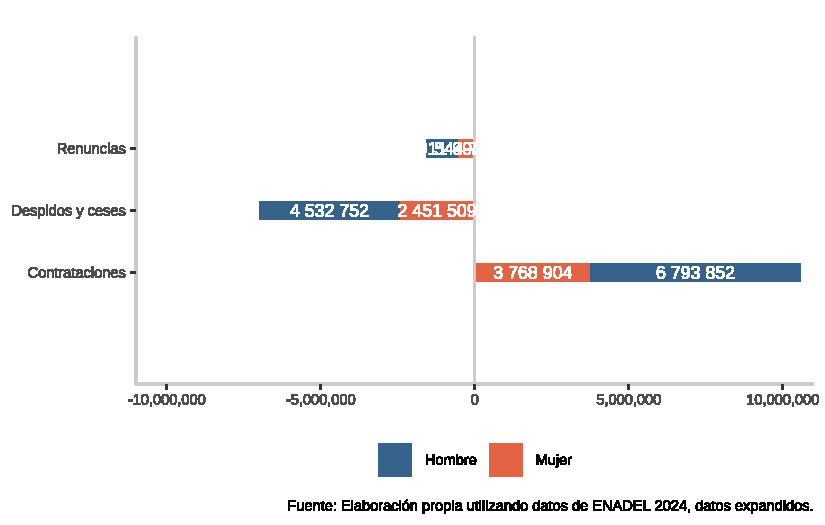
\includegraphics[width=1\textwidth,height=\textheight]{reporte_2024_files/figure-pdf/fig-salidas_contrataciones-1.pdf}

}

\end{figure}%

La Tabla~\ref{tbl-vacantes_region} muestra los cargos u ocupaciones que
las empresas no lograron cubrir durante los últimos doce meses,
desglosados por región, indicando la ocupación con más vacantes dentro
de cada región. La región Los Lagos registra la ocupación Otros
operarios de la construcción (obra gruesa) no clasificados previamente
omo la que cuenta con la mayor cantidad de vacantes sin llenar (362) a
nivel nacional. En la región Metropolitana la ocupación Obreros de la
construcción de edificios tuvo 322 puestos de trabajo sin cubrir. En
tercer lugar, la región con más ocupaciones de difícil cobertura fue
Ñuble, cuya ocupación con más vacantes fue Obreros de explotaciones
agrícolas con 283 vacantes.

\begin{table}

\caption{\label{tbl-vacantes_region}Vacantes por región}

\centering{

\centering
\begin{tabular}{>{\raggedright\arraybackslash}p{4cm}>{\raggedright\arraybackslash}p{7cm}>{\raggedleft\arraybackslash}p{2cm}>{\raggedright\arraybackslash}p{2cm}}
\toprule
Región & Glosa & Vacantes & CV\\
\midrule
Valparaíso & Guardias de seguridad & 165 & 71,1\%\\
O'Higgins & Vendedores de entradas (entretenciones y eventos deportivos) y cajeros de comercio & 213 & 72,2\%\\
Biobío & Ingenieros civiles, ingenieros en construcción y constructores civiles & 240 & 79,7\%\\
Los Lagos & Otros operarios de la construcción (obra gruesa) no clasificados previamente & 362 & 62,7\%\\
Metropolitana & Obreros de la construcción de edificios & 322 & 65,5\%\\
\addlinespace
Arica y Parinacota & Guardias de seguridad & 128 & 71,6\%\\
Ñuble & Obreros de explotaciones agrícolas & 283 & 49,8\%\\
\bottomrule
\multicolumn{4}{l}{\rule{0pt}{1em}Fuente: Elaboración propia utilizando datos de ENADEL 2024.}\\
\end{tabular}

}

\end{table}%

La Tabla~\ref{tbl-vacantes_sector} detalla los cargos u ocupaciones que
las empresas no lograron cubrir durante los últimos doce meses,
organizados según el sector de actividad económica. Dentro de este
análisis, el sector Agricultura, silvicultura y pesca destaca por tener
la mayor cantidad de vacantes sin llenar a nivel nacional en la
ocupación Obreros de la construcción de edificios, con un total de 566
puestos. En la región Industrias manufactureras, la ocupación con más
vacantes fue Obreros de explotaciones agrícolas, acumulando 563
posiciones sin cubrir. Por su parte, la región Comercio se ubicó en
tercer lugar, con la ocupación Guardias de seguridad registrando 430
vacantes disponibles.

\begin{table}

\caption{\label{tbl-vacantes_sector}Vacantes por sector de actividad
económica}

\centering{

\centering
\begin{tabular}{>{\raggedright\arraybackslash}p{4cm}>{\raggedright\arraybackslash}p{7cm}>{\raggedleft\arraybackslash}p{2cm}>{\raggedright\arraybackslash}p{2cm}}
\toprule
Sector de actividad económica & Glosa & Vacantes & CV\\
\midrule
Agricultura, silvicultura y pesca & Obreros de la construcción de edificios & 566 & 87,1\%\\
Industrias manufactureras & Obreros de explotaciones agrícolas & 563 & 64,7\%\\
Suministro de electricidad y gas & Reguladores y operarios de máquinas herramientas & 98 & 100\%\\
Suministro de agua y gestión de  desechos & Otros operarios de la construcción (obra gruesa) no clasificados previamente & 397 & 100\%\\
Construcción & Obreros de la construcción de edificios & 278 & 69,5\%\\
\addlinespace
Comercio & Guardias de seguridad & 430 & 58,3\%\\
Transporte y almacenamiento & Guardias de seguridad & 161 & 71,4\%\\
Alojamiento y de servicio de comida & Directores, gerentes y administradores de recursos humanos & 297 & 100\%\\
Información y comunicaciones & Conductores de camiones pesados y de alto tonelaje & 108 & 90,1\%\\
Actividades financieras y de seguros & Ayudantes de cocina & 74 & 100\%\\
\addlinespace
Actividades inmobiliarias & Obreros de explotaciones agrícolas & 155 & 60,5\%\\
Actividades profesionales y técnicas & Bármanes & 283 & 100\%\\
Servicios administrativos y de apoyo & Obreros de explotaciones agrícolas & 285 & 48\%\\
Actividades artísticas y recreativas / Otras actividades de servicios & Otras ocupaciones elementales no clasificadas previamente & 293 & 100\%\\
\bottomrule
\multicolumn{4}{l}{\rule{0pt}{1em}Fuente: Elaboración propia utilizando datos de ENADEL 2024.}\\
\end{tabular}

}

\end{table}%

\subsection{Ocupaciones de Difícil
Cobertura}\label{ocupaciones-de-difuxedcil-cobertura}

Las ocupaciones de difícil cobertura son aquellas ocupaciones o puestos
de trabajo que los empleadores encuentran difíciles de cubrirpor
diferentes causas como la escasez de trabajadores con las competencias,
habilidades o experiencia necesarias. Estas dificultades pueden
originarse por la falta de oferta de mano de obra calificada, brechas de
habilidades técnicas o blandas, condiciones laborales poco atractivas
(como salarios bajos o jornadas extensas), o problemas de localización
geográfica que limitan el acceso a trabajadores en regiones específicas.
Identificar estas ocupaciones permite entender las dinámicas del mercado
laboral y los desafíos que enfrentan distintos sectores productivos del
país.

Medir este tipo de ocupaciones es fundamental porque facilita el
emparejamiento (\textbf{match}) entre la oferta y la demanda laboral,
orientando programas de capacitación y formación hacia las necesidades
reales del mercado. Además, ayuda a optimizar los procesos de
intermediación laboral y permite anticipar tendencias, ayudando a
trabajadores y estudiantes a tomar decisiones informadas sobre su
desarrollo profesional. Al mismo tiempo, contribuye a reducir
desigualdades regionales al focalizar esfuerzos en zonas rezagadas,
fortaleciendo el capital humano y mejorando la competitividad del país.
En síntesis, esta medición es clave para implementar políticas públicas
más efectivas y promover una fuerza laboral adaptada a los desafíos
económicos actuales y futuros.

La Tabla~\ref{tbl-cuadro8_odc} sólo muestra aquellas para las cuáles el
coeficiente de variación es menor a 40\%\footnote{La convención es
  considerar cómo robustas estimaciones con un cv menor al 15\%. Dado
  que esto no se cumple, se presentan todas las ocupaciones con un cv
  menor a 40\%.}. Durante los últimos 12 meses, el total de vacantes que
no se pudieron llenar fueron de 200,045 vacantes, de las cuales, la
ocupación más difícil de cubrir fue la de Obreros de explotaciones
agrícolas con un total de 1.827 vacantes sin llenar. En segundo lugar,
la ocupación Obreros de la construcción de edificios tuvo un total de
1.438 vacantes sin llenar. Y La ocupación de Guardias de seguridad tuvo
un total de 1.117 vacantes sin cubrir.

\begin{table}

\caption{\label{tbl-cuadro8_odc}Ocupaciones de difícil cobertura, ENADEL
2024.}

\centering{

\centering
\begin{tabular}{r>{\raggedright\arraybackslash}p{9cm}ll}
\toprule
CIUO 08 & Glosa & Vacantes & CV\\
\midrule
9211 & Obreros de explotaciones agrícolas & 1.827 & 25,5\%\\
9313 & Obreros de la construcción de edificios & 1.438 & 39,8\%\\
5414 & Guardias de seguridad & 1.117 & 29,6\%\\
5230 & Vendedores de entradas (entretenciones y eventos deportivos) y cajeros de comercio & 1.044 & 28,9\%\\
9412 & Ayudantes de cocina & 915 & 30,6\%\\
\addlinespace
5131 & Garzones de mesa & 849 & 29,1\%\\
5223 & Vendedores y asistentes de venta de tiendas, almacenes y puestos de mercado & 684 & 34,2\%\\
4110 & Trabajadores de tareas administrativas generales & 553 & 38,6\%\\
7233 & Mecánicos y reparadores de máquinas agrícolas e industriales & 513 & 36,9\%\\
3123 & Supervisores de la construcción & 512 & 37,5\%\\
\addlinespace
7212 & Soldadores y oxicortadores & 480 & 32,6\%\\
4321 & Empleados encargados del control de abastecimiento e inventario & 444 & 39,1\%\\
5245 & Bomberos de gasolineras & -3.637 & -101,9\%\\
8332 & Conductores de camiones pesados y de alto tonelaje & -7.785 & -108,4\%\\
8342 & Operadores de máquinas de movimiento de tierras & -8.066 & -102,4\%\\
\bottomrule
\multicolumn{4}{l}{\rule{0pt}{1em}Fuente: Elaboración propia utilizando datos de ENADEL 2024.}\\
\end{tabular}

}

\end{table}%

La Tabla~\ref{tbl-odc_dummy_sector} indica la cantidad y proporción de
empresas que tuvieron vacantes sin llenar durante los últimos doce meses
diferenciando por sector de actividad económica, en la tabla se aprecia
que la actividad económica con mayor proporción de empresas con vacantes
sin llenar fue el sector Suministro de electricidad y gas (15,9\%). En
segundo lugar, dentro del sector de Actividades artísticas y recreativas
/ Otras actividades de servicios. el 14,9\% de las empresas registró
ocupaciones de difícil cobertura. El tercer sector de actividad
económica con mayor proporción de empresas que afirman tener ocupaciones
dificiles de cubrir fue Suministro de agua y gestión de desechos con 675
empresas equivalente al 11,9\% del total de empresas del sector.

En cambio, los sectores de actividad económica con menor proporción de
empresas que afirmaron tener vacantes sin llenar fueron los sectores de
Servicios administrativos y de apoyo, Actividades inmobiliarias y
Actividades financieras y de seguros con menos del 7,7\% de empresas que
registraron ocupaciones dificiles de cubrir.

\begin{table}

\caption{\label{tbl-odc_dummy_sector}Empresas con ocupaciones de díficil
cobertura según sector de actividad económica}

\centering{

\centering
\begin{tabular}{>{\raggedright\arraybackslash}p{6cm}>{\raggedright\arraybackslash}p{2cm}>{\raggedright\arraybackslash}p{2cm}>{\raggedright\arraybackslash}p{1.5cm}>{\raggedright\arraybackslash}p{1.5cm}l}
\toprule
Sector de actividad económica & Sí & No & Total empresas & \% Sí & \% No\\
\midrule
Suministro de electricidad y gas & 419 & 2.211 & 2.630 & 15,9\% & 84,1\%\\
Actividades artísticas y recreativas / Otras actividades de servicios. & 1.042 & 5.939 & 6.982 & 14,9\% & 85,1\%\\
Suministro de agua y gestión de  desechos & 675 & 4.980 & 5.655 & 11,9\% & 88,1\%\\
Actividades profesionales y técnicas & 1.366 & 10.538 & 11.904 & 11,5\% & 88,5\%\\
Industrias manufactureras & 3.095 & 24.230 & 27.324 & 11,3\% & 88,7\%\\
\addlinespace
Información y comunicaciones & 974 & 7.771 & 8.745 & 11,1\% & 88,9\%\\
Construcción & 2.644 & 21.626 & 24.270 & 10,9\% & 89,1\%\\
Agricultura, silvicultura y pesca & 2.209 & 19.878 & 22.087 & 10\% & 90\%\\
Comercio & 4.264 & 42.287 & 46.551 & 9,2\% & 90,8\%\\
Alojamiento y de servicio de comida & 2.978 & 32.096 & 35.075 & 8,5\% & 91,5\%\\
\addlinespace
Transporte y almacenamiento & 1.898 & 21.057 & 22.955 & 8,3\% & 91,7\%\\
Servicios administrativos y de apoyo & 1.569 & 18.784 & 20.353 & 7,7\% & 92,3\%\\
Actividades inmobiliarias & 514 & 7.363 & 7.877 & 6,5\% & 93,5\%\\
Actividades financieras y de seguros & 119 & 2.811 & 2.931 & 4,1\% & 95,9\%\\
\bottomrule
\multicolumn{6}{l}{\rule{0pt}{1em}Fuente: Elaboración propia utilizando datos de ENADEL 2024.}\\
\end{tabular}

}

\end{table}%

Al analizar cada sector económico, se identificaron las ocupaciones con
mayor cantidad de vacantes sin cubrir. El sector económico de
Agricultura, silvicultura y pesca registró Obreros de la construcción de
edificios como la ocupación con más vacantes de dícifil cobertura con un
total de 566 puestos de trabajos sin llenar. En segundo lugar, dentro
del sector de actividad Industrias manufactureras la ocupación Obreros
de explotaciones agrícolas tuvo 563 vacantes sin llenar. Para el sector
de Comercio la ocupación con más vacantes de díficil cobertura fue
Guardias de seguridad con un total de 430 puestos de trabajo sin llenar.
Por otro lado, los sectores con menores vacantes sin llenar fueron
Información y comunicaciones,Suministro de electricidad y gas y
Actividades financieras y de seguros en la Figura~\ref{fig-odc_sector}
se observa que las ocupaciones de estos sectores fueron Conductores de
camiones pesados y de alto tonelaje, Reguladores y operarios de máquinas
herramientas y Ayudantes de cocina con 108 o menos puestos de trabajo
sin cubrir.

\begin{figure}[H]

\caption{\label{fig-odc_sector}Cantidad de ocupaciones de díficil
cobertura por sector de actividad económica}

\centering{

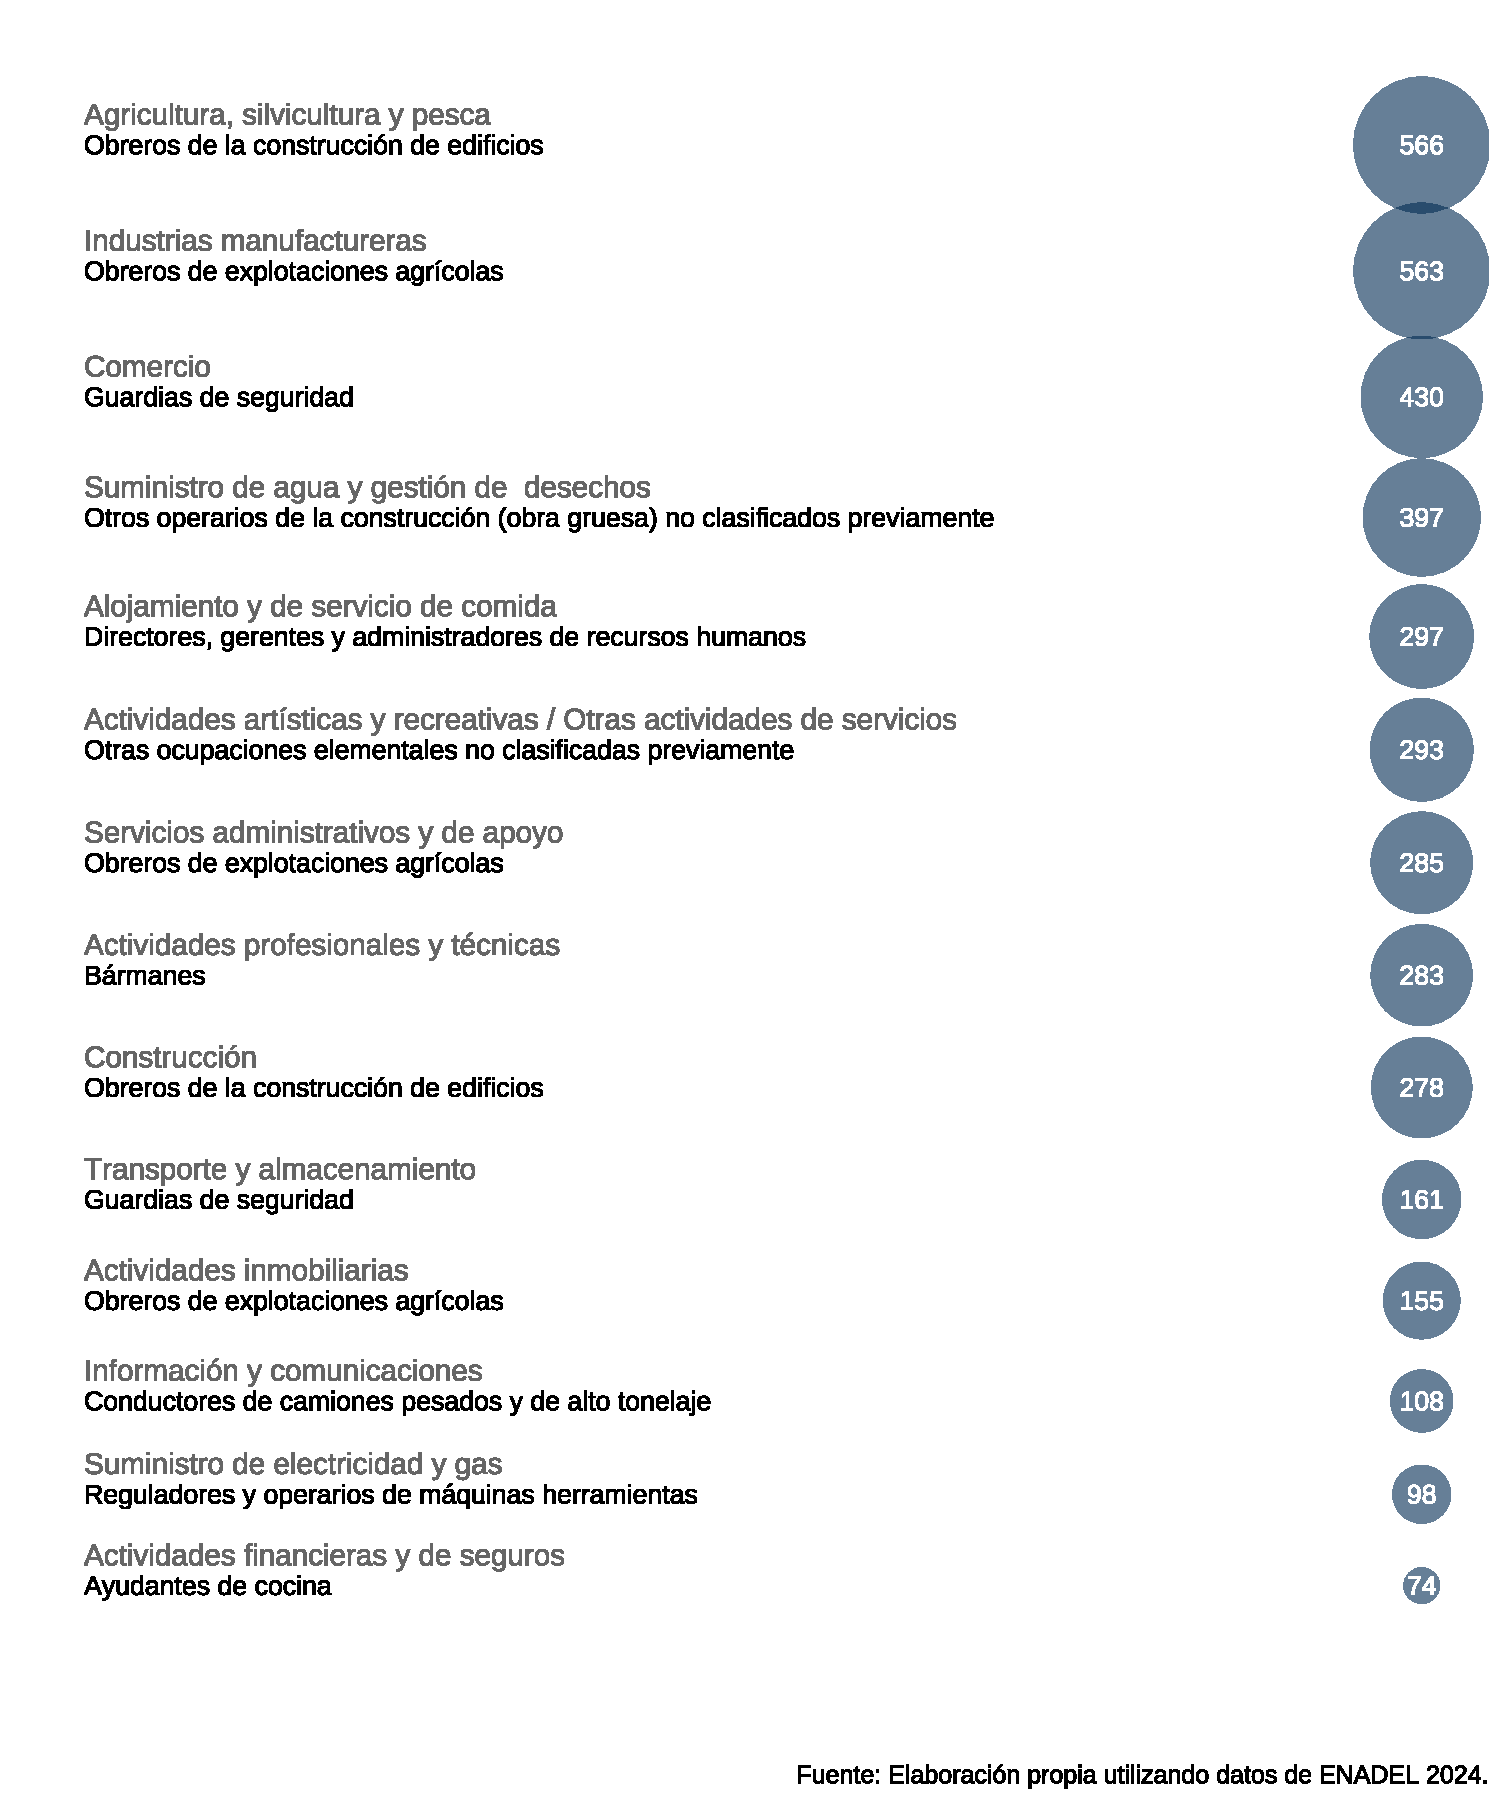
\includegraphics[width=1\textwidth,height=\textheight]{reporte_2024_files/figure-pdf/fig-odc_sector-1.pdf}

}

\end{figure}%

La Tabla~\ref{tbl-odc_dummy_region} indica la cantidad y proporción de
empresas que tuvieron vacantes sin llenar durante los últimos doce meses
diferenciando por región, en la tabla se aprecia que la región con mayor
proporción de empresas con vacantes sin llenar fue la región Tarapacá
(19\%). En segundo lugar, dentro de la región de Coquimbo el 16,3\% de
las empresas registró ocupaciones de difícil cobertura. La tercera
región con mayor proporción de empresas que afirman tener ocupaciones
dificiles de cubrir fue Metropolitana con 1.922 empresas equivalente al
16,2\% del total de empresas de la región.

En cambio, las regiones con menor proporción de empresas que afirmaron
tener vacantes sin llenar fueron Maule, O'Higgins y Arica y Parinacota
con menos del 7\% de empresas que registraron ocupaciones dificiles de
cubrir.

\begin{table}

\caption{\label{tbl-odc_dummy_region}Empresas con ocupaciones de díficil
cobertura por región}

\centering{

\centering
\begin{tabular}{>{\raggedright\arraybackslash}p{4cm}>{\raggedright\arraybackslash}p{2cm}>{\raggedright\arraybackslash}p{2cm}>{\raggedright\arraybackslash}p{1.5cm}>{\raggedright\arraybackslash}p{1.5cm}l}
\toprule
Región & Sí & No & Total empresas & \% Sí & \% No\\
\midrule
Arica y Parinacota & 554 & 8.982 & 9.536 & 5,8\% & 94,2\%\\
Tarapacá & 1.496 & 6.369 & 7.865 & 19\% & 81\%\\
Antofagasta & 1.119 & 6.067 & 7.185 & 15,6\% & 84,4\%\\
Atacama & 1.610 & 9.974 & 11.583 & 13,9\% & 86,1\%\\
Coquimbo & 2.004 & 10.290 & 12.294 & 16,3\% & 83,7\%\\
\addlinespace
Valparaíso & 1.190 & 19.979 & 21.170 & 5,6\% & 94,4\%\\
Metropolitana & 1.922 & 9.946 & 11.868 & 16,2\% & 83,8\%\\
O'Higgins & 1.064 & 16.824 & 17.887 & 5,9\% & 94,1\%\\
Maule & 1.696 & 22.532 & 24.228 & 7\% & 93\%\\
Ñuble & 2.257 & 15.070 & 17.327 & 13\% & 87\%\\
\addlinespace
Biobío & 2.434 & 24.552 & 26.986 & 9\% & 91\%\\
La Araucanía & 1.574 & 18.761 & 20.334 & 7,7\% & 92,3\%\\
Los Ríos & 630 & 16.488 & 17.118 & 3,7\% & 96,3\%\\
Los Lagos & 2.314 & 21.702 & 24.016 & 9,6\% & 90,4\%\\
Aysén & 764 & 4.902 & 5.666 & 13,5\% & 86,5\%\\
\addlinespace
Magallanes & 1.141 & 9.137 & 10.277 & 11,1\% & 88,9\%\\
\bottomrule
\multicolumn{6}{l}{\rule{0pt}{1em}Fuente: Elaboración propia utilizando datos de ENADEL 2024.}\\
\end{tabular}

}

\end{table}%

La Tabla~\ref{tbl-odc_region} muestra las ocupaciones más dificiles de
cubrir dentro de cada región, la región con más ocupaciones de difícil
cobertura fue Arica y Parinacota y el puesto de trabajo con más vacantes
sin llenar fue Guardias de seguridad con un total de 128 puestos de
trabajo sin cubrir. La segunda región con más ocupaciones sin llenar fue
Valparaíso cuyo oficio de más vacantes sin llenar fue Guardias de
seguridad con 165 vacantes. Luego, la región Tarapacá registró
Directores, gerentes y administradores de servicios de salud como el
puesto de trabajo de más difícil cobertura con 178 vacantes sin llenar.
Las regiones que registraron menos cantidad de vacantes de difícil
cobertura corresponden a las regiones Los Ríos, La Araucanía y Aysén,
cuyos oficios con más dificultad de cobertura fueron Carpinteros de obra
(365 vacantes), Otros operarios de la construcción (obra gruesa) no
clasificados previamente (397 vacantes) y Obreros de la construcción de
edificios (554 vacantes).

\begin{table}

\caption{\label{tbl-odc_region}Cantidad de ocupaciones de díficil
cobertura por región}

\centering{

\centering
\begin{tabular}{>{\raggedright\arraybackslash}p{4cm}>{\raggedright\arraybackslash}p{7cm}>{\raggedleft\arraybackslash}p{2cm}>{\raggedright\arraybackslash}p{1.5cm}}
\toprule
Región & Glosa & Total vacantes & CV\\
\midrule
Arica y Parinacota & Guardias de seguridad & 128 & 71,6\%\\
Tarapacá & Directores, gerentes y administradores de servicios de salud & 178 & 100\%\\
Antofagasta & Obreros forestales & 335 & 100\%\\
Atacama & Directores, gerentes y administradores de recursos humanos & 297 & 100\%\\
Coquimbo & Otras ocupaciones elementales no clasificadas previamente & 293 & 100\%\\
\addlinespace
Valparaíso & Guardias de seguridad & 165 & 71,1\%\\
Metropolitana & Obreros de la construcción de edificios & 322 & 65,5\%\\
O'Higgins & Vendedores de entradas (entretenciones y eventos deportivos) y cajeros de comercio & 213 & 72,2\%\\
Maule & Técnicos de radiodifusión y grabación audiovisual & 220 & 100\%\\
Ñuble & Obreros de explotaciones agrícolas & 283 & 49,8\%\\
\addlinespace
Biobío & Ingenieros civiles, ingenieros en construcción y constructores civiles & 240 & 79,7\%\\
La Araucanía & Otros operarios de la construcción (obra gruesa) no clasificados previamente & 397 & 100\%\\
Los Ríos & Carpinteros de obra & 365 & 100\%\\
Los Lagos & Otros operarios de la construcción (obra gruesa) no clasificados previamente & 362 & 62,7\%\\
Aysén & Obreros de la construcción de edificios & 554 & 88,7\%\\
\addlinespace
Magallanes & Capitanes y oficiales de cubierta & 262 & 100\%\\
\bottomrule
\multicolumn{4}{l}{\rule{0pt}{1em}Fuente: Elaboración propia utilizando datos de ENADEL 2024.}\\
\end{tabular}

}

\end{table}%

\newpage

\subsection{Principales Dificultades}\label{principales-dificultades}

La Tabla~\ref{tbl-dificultad} muestra las principales dificultades de
contratación. La dificultad más reportada es la de ``Candidatos sin
competencias o habilidades técnicas requeridas'', presente en el
\text{26}\% de los casos, seguida por ``Falta de postulantes'' con un
\text{23,4}\% y ``Condiciones laborales (ubicación, horario y/o jornada)
no aceptadas'', que representa el \text{10}\% del total de los
principales cargos con dificultades de contratación.

\begin{table}

\caption{\label{tbl-dificultad}Dificultades de contratación.}

\centering{

\centering
\begin{tabular}{>{\raggedright\arraybackslash}p{10cm}>{\raggedright\arraybackslash}p{3cm}>{\raggedright\arraybackslash}p{3cm}}
\toprule
Primera dificultad & \% de 1ra dificultad & \% del total\\
\midrule
Candidatos sin competencias o habilidades técnicas requeridas & 24,7\% & 26\%\\
Falta de postulantes & 23,7\% & 23,4\%\\
Condiciones laborales (ubicación, horario y/o jornada) no aceptadas & 10\% & 10\%\\
Otra dificultad & 9\% & 9,5\%\\
Candidatos sin la experiencia mínima requerida & 9,5\% & 8,6\%\\
\addlinespace
Renumeración ofrecida no aceptada & 8,8\% & 8,3\%\\
Candidatos sin habilidades blandas o socioemocionales requeridas & 7,1\% & 7,1\%\\
Candidatos sin licencias, certificaciones o requisitos legales & 5,6\% & 5,3\%\\
Candidatos sin nivel educacional requerido & 1,7\% & 1,8\%\\
\bottomrule
\multicolumn{3}{l}{\rule{0pt}{1em}Fuente: Elaboración propia utilizando datos de ENADEL 2024.}\\
\end{tabular}

}

\end{table}%

\newpage

\section{Capítulo III: Capacitación y
Habilidades}\label{capuxedtulo-iii-capacitaciuxf3n-y-habilidades}

Este capítulo tiene como objetivo identificar las prioridades de
capacitación e inversión en desarrollo de habilidades por parte de las
empresas, así como las ocupaciones que requieren formación específica.
En primer lugar, se analiza la adhesión de las empresas a los Organismos
Técnicos Intermedios para la Capacitación (OTIC) y se evalúa si han
proporcionado efectivamente capacitaciones laborales. Además, se
examinan las competencias que necesitan ser fortalecidas, las fuentes de
financiamiento utilizadas para dichas capacitaciones, así como las
necesidades actuales y las expectativas futuras en materia de formación
laboral.

\subsection{Organismo Técnico Intermedio para
capacitación}\label{organismo-tuxe9cnico-intermedio-para-capacitaciuxf3n}

La Figura~\ref{fig-otic} muestra los porcentajes de empresas que poseen
afiliación a algún Organismo Técnico Intermedio para la Capacitación
(OTIC), en el gráfico se indica que sólo el 18\% de las empresas están
adheridas a un OTIC, mientras que el 80,4\% de las organizaciones no
posee adherencia a este tipo de organismos de capacitación.

\begin{figure}[H]

\caption{\label{fig-otic}Empresas adheridas a Organismo Técnico
Intermedio para Capacitación (OTIC)}

\centering{

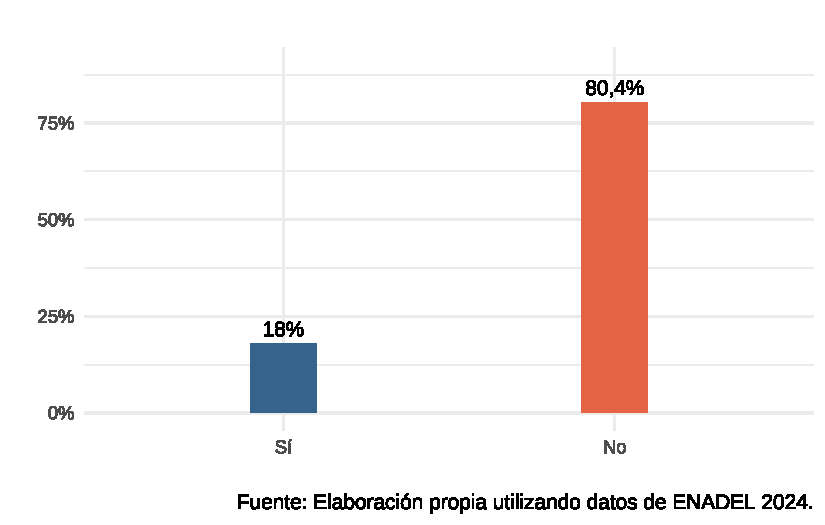
\includegraphics{reporte_2024_files/figure-pdf/fig-otic-1.pdf}

}

\end{figure}%

\newpage

\subsection{Capacitaciones de la
empresa}\label{capacitaciones-de-la-empresa}

Con respecto a la distribución de las empresas que trabajan con algún
OTIC, la tabla Tabla~\ref{tbl-otic_sector} clasifica a las empresas
según su adhesión a un organismo técnico de capacitación y el sector de
actividad económica al que pertenecen. El sector de actividad económica
que mayor cantidad de empresas asociadas a un OTIC es el sector Comercio
con un total de 7.397 empresas. Sin embargo, estas representan sólo el
16,2\% de empresas de este sector económico. El sector de actividad
económica con mayor proporción de empresas adheridas a algún OTIC es el
sector de Actividades financieras y de seguros con un total de 1.035
empresas que representan el 35,9\% de las empresas de este sector.

El sector con menor cantidad de organizaciones afiliadas a algún
organismo intermedio de capacitación es Suministro de electricidad y gas
con 760 empresas adheridas a algún OTIC, equivalente al 28,9\% de
organizaciones. Mientras que el sector con menor proporción de empresas
adheridas a un OTIC es Alojamiento y de servicio de comida con sólo el
10,9\% de sus empresas que trabajan con algún organismo de capacitación,
equivalente a 3.760. empresas.

\begin{table}

\caption{\label{tbl-otic_sector}Empresas adheridas a Organismo Técnico
Intermedio para Capacitación (OTIC) según sector económico}

\centering{

\centering
\begin{tabular}{>{\raggedright\arraybackslash}p{6cm}>{\raggedright\arraybackslash}p{2cm}>{\raggedright\arraybackslash}p{2cm}>{\raggedright\arraybackslash}p{2cm}ll}
\toprule
Sector de Actividad Económica & Sí & No & Total empresas & \% Sí & \% No\\
\midrule
Comercio & 7.397 & 38.252 & 45.649 & 16,2\% & 83,8\%\\
Industrias manufactureras & 5.340 & 21.627 & 26.967 & 19,8\% & 80,2\%\\
Agricultura, silvicultura y pesca & 5.277 & 16.445 & 21.722 & 24,3\% & 75,7\%\\
Construcción & 5.219 & 18.788 & 24.008 & 21,7\% & 78,3\%\\
Servicios administrativos y de apoyo & 4.527 & 15.627 & 20.153 & 22,5\% & 77,5\%\\
\addlinespace
Transporte y almacenamiento & 3.821 & 18.802 & 22.623 & 16,9\% & 83,1\%\\
Alojamiento y de servicio de comida & 3.760 & 30.771 & 34.532 & 10,9\% & 89,1\%\\
Actividades inmobiliarias & 1.844 & 6.033 & 7.877 & 23,4\% & 76,6\%\\
Actividades profesionales y técnicas & 1.482 & 10.081 & 11.563 & 12,8\% & 87,2\%\\
Suministro de agua y gestión de  desechos & 1.290 & 4.174 & 5.465 & 23,6\% & 76,4\%\\
\addlinespace
Actividades artísticas y recreativas / Otras actividades de servicios. & 1.228 & 5.577 & 6.805 & 18\% & 82\%\\
Información y comunicaciones & 1.213 & 7.478 & 8.691 & 14\% & 86\%\\
Actividades financieras y de seguros & 1.035 & 1.847 & 2.881 & 35,9\% & 64,1\%\\
Suministro de electricidad y gas & 760 & 1.869 & 2.630 & 28,9\% & 71,1\%\\
\bottomrule
\multicolumn{6}{l}{\rule{0pt}{1em}Fuente: Elaboración propia utilizando datos de ENADEL 2024.}\\
\end{tabular}

}

\end{table}%

\newpage

La Tabla~\ref{tbl-otic_region} presenta la distribución de las empresas
según su adhesión a un OTIC y a la región donde se ubican. La región con
mayor cantidad de empresas adheridas a un OTIC es la región del Maule
con un total de 5.153 empresas, lo que equivale al 22\% de las empresas
de la región. En cuanto al porcentaje de empresas afiliadas a un OTIC,
la región de Antofagasta presenta la mayor proporción de empresas de la
región con adherencia a un OTIC con un total de 1797 equivalente al
29,9\% del total de organizaciones de la región.

La región con menor cantidad de organizaciones afiliadas a algún
organismo intermedio de capacitación es Magallanes con 1.478 empresas
adheridas a algún OTIC, equivalente al 14,8\% de organizaciones.
Mientras que la región con menor proporción de empresas adheridas a un
OTIC es Tarapacá con sólo el 12,7\% de sus empresas que trabajan con
algún organismo de capacitación, equivalente a 977. empresas.

\begin{table}

\caption{\label{tbl-otic_region}Empresas adheridas a Organismo Técnico
Intermedio para Capacitación (OTIC) según Región}

\centering{

\centering
\begin{tabular}{>{\raggedright\arraybackslash}p{6cm}>{\raggedright\arraybackslash}p{2cm}>{\raggedright\arraybackslash}p{2cm}>{\raggedright\arraybackslash}p{2cm}ll}
\toprule
Región & Sí & No & Total empresas & \% Sí & \% No\\
\midrule
Maule & 5.153 & 18.270 & 18.270 & 22\% & 78\%\\
O'Higgins & 4.950 & 12.905 & 12.905 & 27,7\% & 72,3\%\\
Biobío & 4.839 & 21.635 & 21.635 & 18,3\% & 81,7\%\\
Los Lagos & 4.010 & 20.005 & 20.005 & 16,7\% & 83,3\%\\
Metropolitana & 3.263 & 8.448 & 8.448 & 27,9\% & 72,1\%\\
\addlinespace
La Araucanía & 3.245 & 16.914 & 16.914 & 16,1\% & 83,9\%\\
Atacama & 2.804 & 8.779 & 8.779 & 24,2\% & 75,8\%\\
Ñuble & 2.611 & 14.680 & 14.680 & 15,1\% & 84,9\%\\
Valparaíso & 2.431 & 18.418 & 18.418 & 11,7\% & 88,3\%\\
Arica y Parinacota & 2.104 & 7.432 & 7.432 & 22,1\% & 77,9\%\\
\addlinespace
Coquimbo & 2.028 & 10.198 & 10.198 & 16,6\% & 83,4\%\\
Antofagasta & 1.797 & 4.223 & 4.223 & 29,9\% & 70,2\%\\
Los Ríos & 1.640 & 15.478 & 15.478 & 9,6\% & 90,4\%\\
Magallanes & 1.478 & 8.477 & 8.477 & 14,8\% & 85,2\%\\
Tarapacá & 977 & 6.709 & 6.709 & 12,7\% & 87,3\%\\
\addlinespace
Aysén & 864 & 4.801 & 4.801 & 15,2\% & 84,7\%\\
\bottomrule
\multicolumn{6}{l}{\rule{0pt}{1em}Fuente: Elaboración propia utilizando datos de ENADEL 2024.}\\
\end{tabular}

}

\end{table}%

\newpage

La Figura~\ref{fig-capacitacion} proporciona información acerca de las
empresas que declaran haber entregado o realizado capacitaciones
laborales para su personal, en el gráfico se visualiza que la mayoría de
las empresas (72,2\%) afirma que ha realizado/proporcionado capacitación
a sus trabajadores, en contraste al 27,3\% que declara no haber
proporcionado ni realizado capacitaciones laborales a su personal.

\begin{figure}[H]

\caption{\label{fig-capacitacion}Proporción de empresas con
capacitaciones laborales para su personal}

\centering{

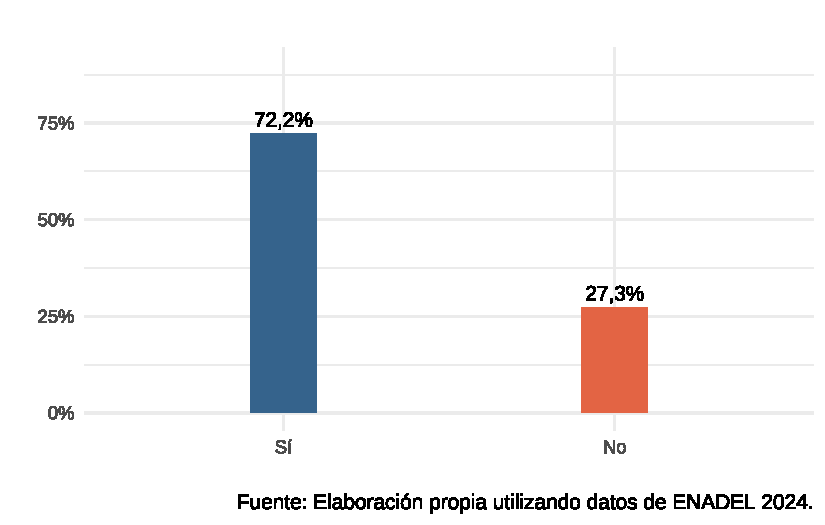
\includegraphics{reporte_2024_files/figure-pdf/fig-capacitacion-1.pdf}

}

\end{figure}%

Al revisar cómo se distribuyen las empresas que realizan capacitaciones
a sus trabajadores según sector de actividad económica, la
Tabla~\ref{tbl-capacitacion_sector} indica que el sector con mayor
cantidad de empresas que aseveran realizar capacitación a sus
trabajadores es el sector Comercio con 30.536 empresas que capacitan a
su personal, lo que equivale al 65,8\% de las empresas del sector de
Comercio. En segundo lugar, el sector Alojamiento y de servicio de
comida cuenta con 24.902 empresas que declaran proporcionan
capacitación, lo que equivale al 71,3\% de empresas del sector. El
tercer sector con más cantidad de empresas que afirman entregar
capacitación a sus trabajadores es Industrias manufactureras con 19.903
organizaciones.

De manera opuesta, en los sectores Suministro de agua y gestión de
desechos, Suministro de electricidad y gas y Actividades financieras y
de seguros hay menor cantidad de empresas que sostienen realizar
capacitaciones a sus trabajadores.

\begin{table}

\caption{\label{tbl-capacitacion_sector}Empresas que proporcionan o
realizan capacitación a su personal según sector económico}

\centering{

\centering
\begin{tabular}{>{\raggedright\arraybackslash}p{6cm}>{\raggedright\arraybackslash}p{2cm}>{\raggedright\arraybackslash}p{2cm}>{\raggedright\arraybackslash}p{2cm}ll}
\toprule
Sector de Actividad Económica & Sí & No & Total empresas & \% Sí & \% No\\
\midrule
Comercio & 30.536 & 15.865 & 46.401 & 65,8\% & 34,2\%\\
Alojamiento y de servicio de comida & 24.902 & 10.006 & 34.908 & 71,3\% & 28,7\%\\
Industrias manufactureras & 19.903 & 7.174 & 27.078 & 73,5\% & 26,5\%\\
Construcción & 18.071 & 6.048 & 24.119 & 74,9\% & 25,1\%\\
Transporte y almacenamiento & 16.846 & 5.899 & 22.744 & 74,1\% & 25,9\%\\
\addlinespace
Agricultura, silvicultura y pesca & 16.798 & 5.257 & 22.055 & 76,2\% & 23,8\%\\
Servicios administrativos y de apoyo & 15.241 & 4.943 & 20.184 & 75,5\% & 24,5\%\\
Actividades profesionales y técnicas & 9.495 & 2.377 & 11.872 & 80\% & 20\%\\
Información y comunicaciones & 6.024 & 2.667 & 8.691 & 69,3\% & 30,7\%\\
Actividades artísticas y recreativas / Otras actividades de servicios. & 5.253 & 1.729 & 6.982 & 75,2\% & 24,8\%\\
\addlinespace
Actividades inmobiliarias & 5.084 & 2.763 & 7.847 & 64,8\% & 35,2\%\\
Suministro de agua y gestión de  desechos & 4.465 & 1.112 & 5.578 & 80\% & 19,9\%\\
Suministro de electricidad y gas & 2.283 & 347 & 2.630 & 86,8\% & 13,2\%\\
Actividades financieras y de seguros & 2.237 & 693 & 2.931 & 76,3\% & 23,6\%\\
\bottomrule
\multicolumn{6}{l}{\rule{0pt}{1em}Fuente: Elaboración propia utilizando datos de ENADEL 2024.}\\
\end{tabular}

}

\end{table}%

Con respecto a la distribución de las empresas que declaran realizar
capacitaciones a su personal según su región de ubicación, la
Tabla~\ref{tbl-capacitacion_region} indica que la región Biobío
concentra la mayor cantidad de empresas (20.170) equivalente a un 75,4\%
de las empresas de la región. En segundo lugar, la región Los Lagos
posee 16.951 empresas (70,6\%) que hacen capacitación. Y en tercer
lugar, la región de Maule cuenta con 15.985 (66,1\%) empresas que
proporcionan capacitaciones a su personal. No obstante, las regiones con
mayor porcentaje de empresas que afirman entregar capacitación son
O'Higgins (80,7\%), Magallanes (80\%) y Atacama (79,6\%).

En cambio, en las regiones de Tarapacá, Antofagasta y Aysén es donde hay
menos empresas que realicen capacitación. Mientras que las regiones que
tienen menor porcentaje de organizaciones que entregan capacitación
corresponden a Arica y Parinacota (66,9\%), Los Ríos (66,8\%) y Maule
(66,1\%).

\begin{table}

\caption{\label{tbl-capacitacion_region}Empresas que proporcionan o
realizan capacitación a su personal según región}

\centering{

\centering
\begin{tabular}{>{\raggedright\arraybackslash}p{6cm}>{\raggedright\arraybackslash}p{2cm}>{\raggedright\arraybackslash}p{2cm}>{\raggedright\arraybackslash}p{2cm}ll}
\toprule
region de Actividad Económica & Sí & No & Total empresas & \% Sí & \% No\\
\midrule
Biobío & 20.170 & 6.566 & 26.736 & 75,4\% & 24,6\%\\
Los Lagos & 16.951 & 7.065 & 24.016 & 70,6\% & 29,4\%\\
Maule & 15.985 & 8.210 & 24.195 & 66,1\% & 33,9\%\\
La Araucanía & 15.098 & 5.236 & 20.334 & 74,3\% & 25,7\%\\
O'Higgins & 14.384 & 3.447 & 17.831 & 80,7\% & 19,3\%\\
\addlinespace
Valparaíso & 14.352 & 6.741 & 21.093 & 68\% & 32\%\\
Ñuble & 12.900 & 4.337 & 17.237 & 74,8\% & 25,2\%\\
Los Ríos & 11.439 & 5.678 & 17.118 & 66,8\% & 33,2\%\\
Metropolitana & 9.247 & 2.523 & 11.770 & 78,6\% & 21,4\%\\
Atacama & 9.218 & 2.366 & 11.583 & 79,6\% & 20,4\%\\
\addlinespace
Coquimbo & 8.230 & 4.064 & 12.294 & 66,9\% & 33,1\%\\
Magallanes & 8.219 & 2.058 & 10.277 & 80\% & 20\%\\
Arica y Parinacota & 6.376 & 3.159 & 9.536 & 66,9\% & 33,1\%\\
Tarapacá & 5.647 & 2.179 & 7.827 & 72,1\% & 27,8\%\\
Antofagasta & 4.896 & 1.608 & 6.504 & 75,3\% & 24,7\%\\
\addlinespace
Aysén & 4.025 & 1.641 & 5.666 & 71\% & 29\%\\
\bottomrule
\multicolumn{6}{l}{\rule{0pt}{1em}Fuente: Elaboración propia utilizando datos de ENADEL 2024.}\\
\end{tabular}

}

\end{table}%

\subsection{Competencias en que se
capacita}\label{competencias-en-que-se-capacita}

La Figura~\ref{fig-competencias_capacitadas} muestra la cantidad de
empresas que realizaron capacitaciones según el tipo de competencia. La
competencia sobre la cual se realizaron más capacitaciones en los
útlimos doce meses corresponde a Competencias técnicas con 119.052
empresas que realizaron este tipo de capacitaciones. En segundo lugar,
116.473 empresas realizaron capacitaciones en Competencias de salud
ocupacional y prevención, seguido de Competencias actitudinales,
conductuales, emocionales y/o valóricas con 64.218 empresas. Por el
contrario, las competencias menos priorizadas para la capacitación según
número de empresas corresponde a Competencias digitales avanzadas con
20.235 empresas y Competencias en idiomas extranjeros con 7.001 empresas
que realizaron este tipo de capacitaciones.

\begin{figure}[H]

\caption{\label{fig-competencias_capacitadas}Competencias en las que se
capacitó a los trabajadores(as)}

\centering{

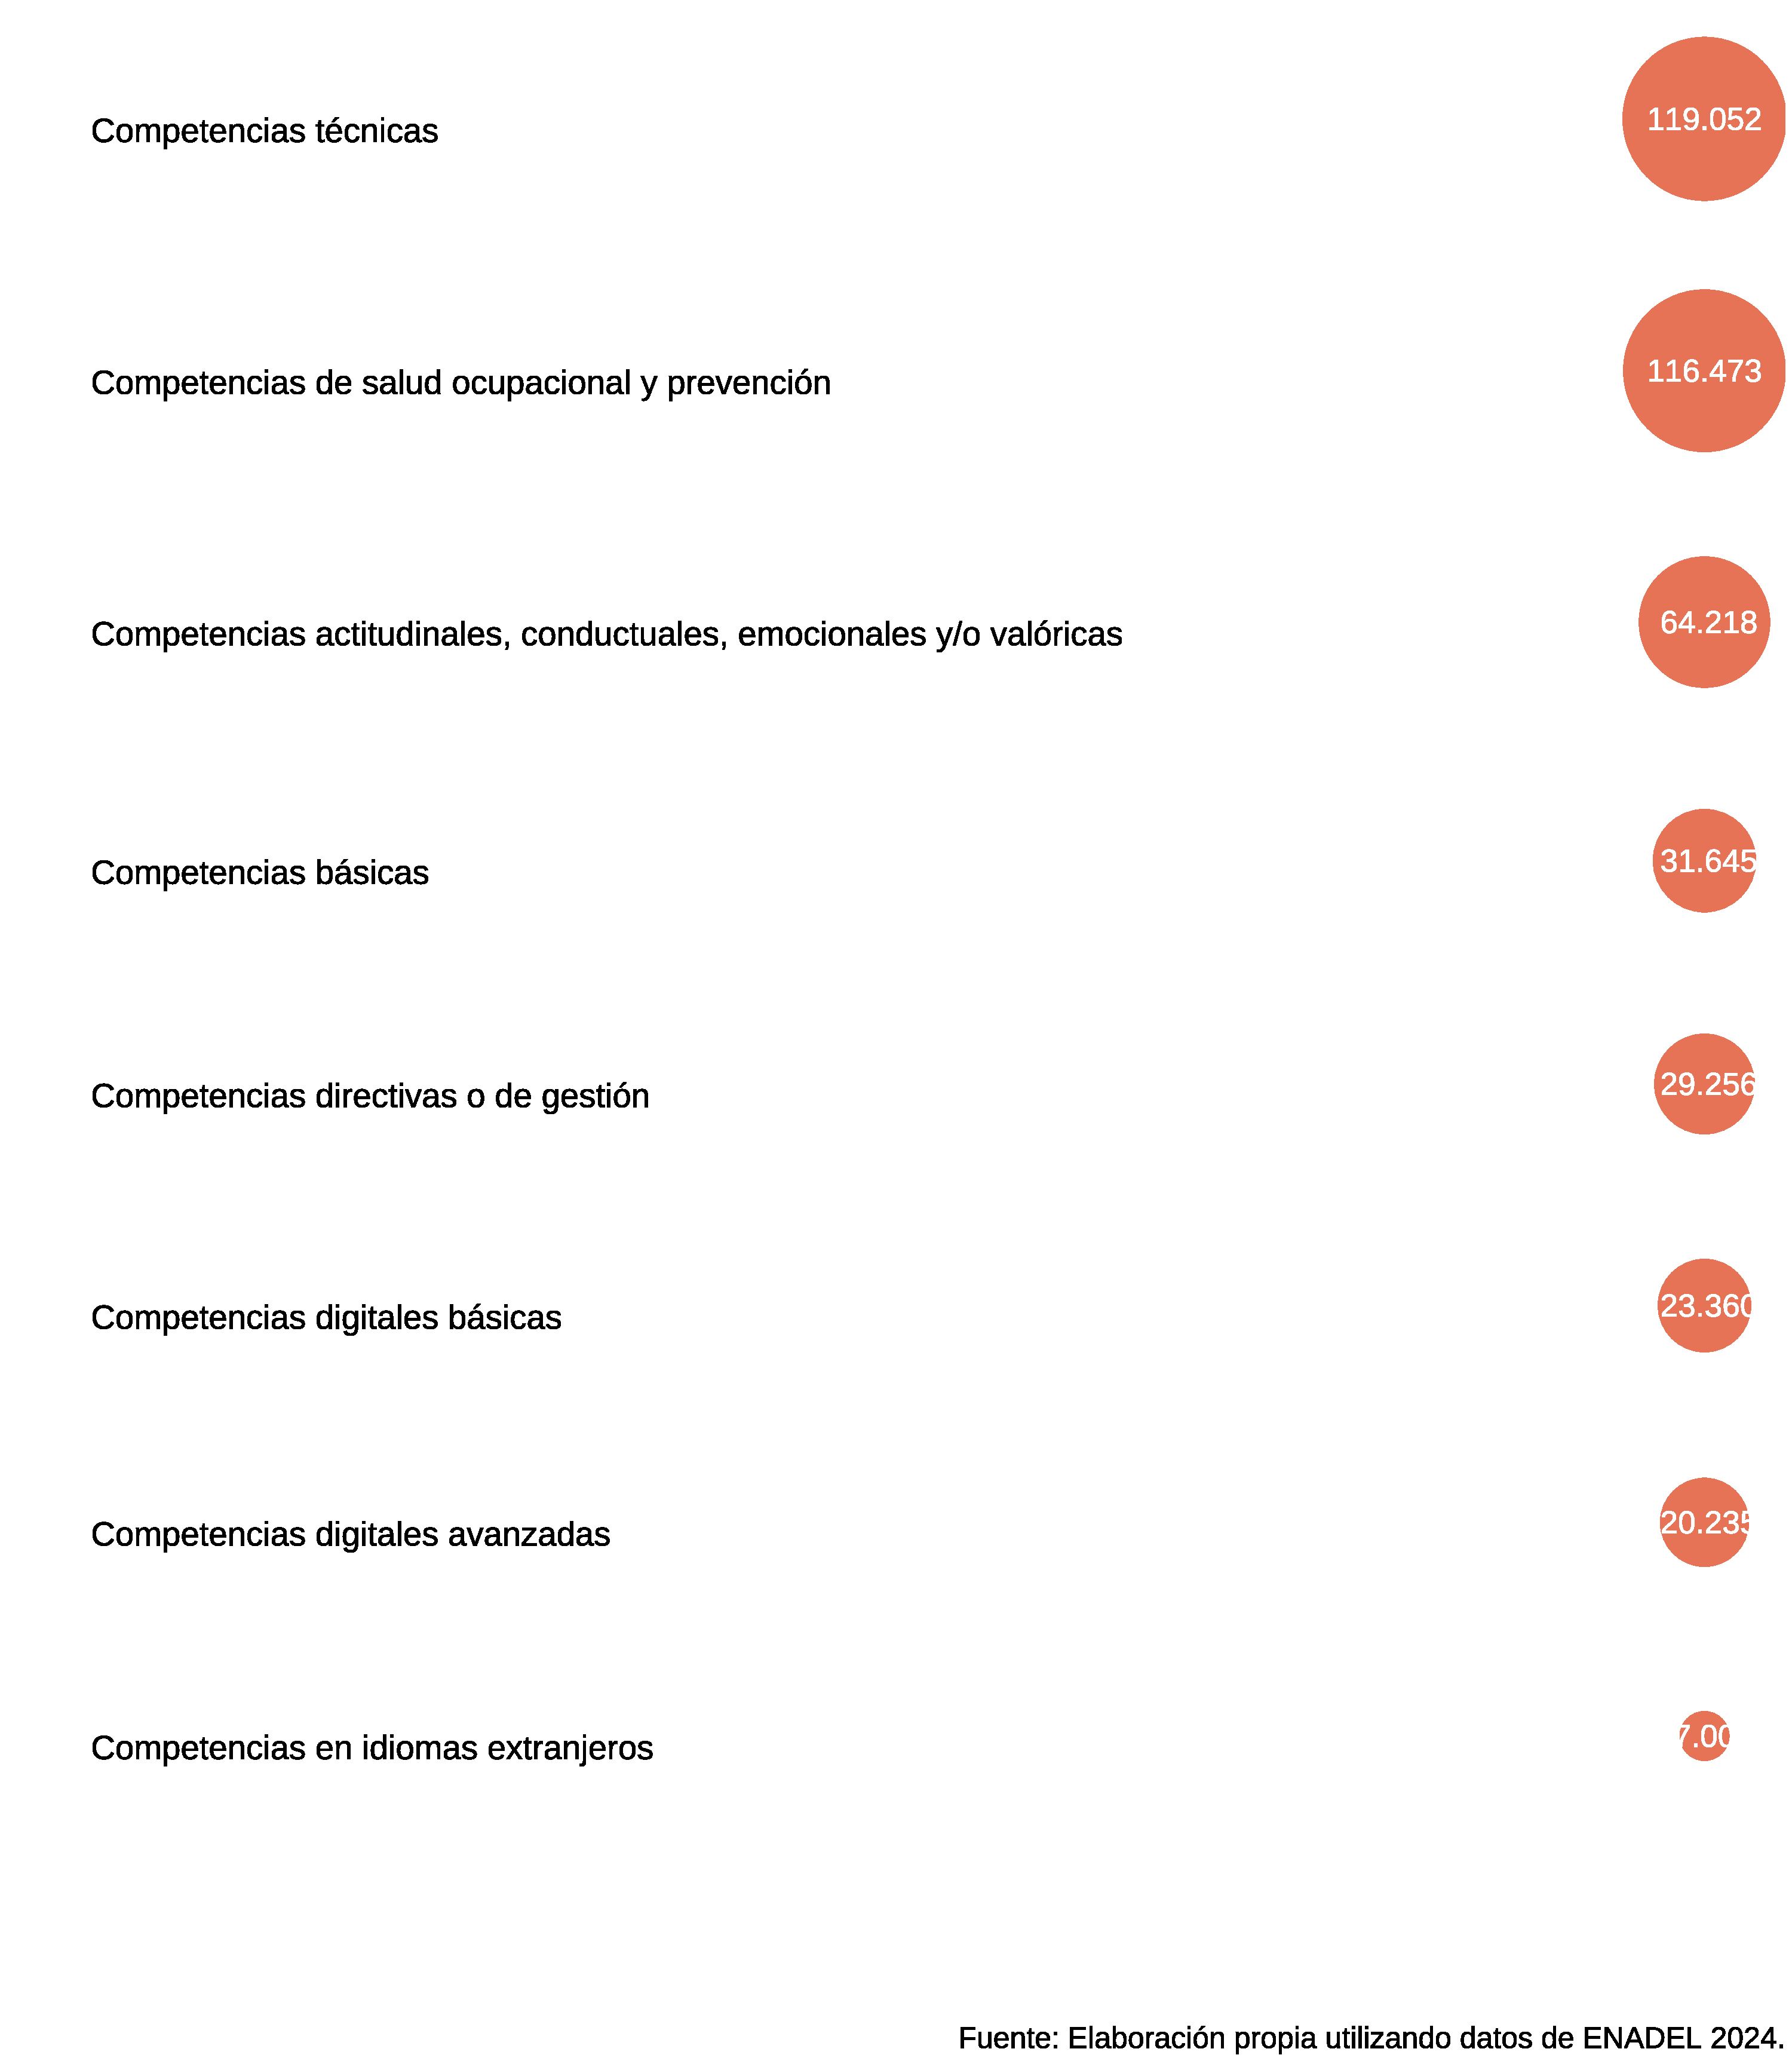
\includegraphics[width=1\textwidth,height=\textheight]{reporte_2024_files/figure-pdf/fig-competencias_capacitadas-1.pdf}

}

\end{figure}%

\newpage

A pesar de no haber ofrecido capacitaciones a sus trabajadores, las
empresas suelen enfrentar la necesidad de ciertas competencias. La
Figura~\ref{fig-competencias_necesarias} ilustra las competencias que
han sido requeridas por las empresas durante los últimos doce meses,
esta tabla muestra la cantidad de empresas que necesitaron
capacitaciones según el tipo de competencia. La competencia más
requerida para capacitaciones en los útlimos doce meses corresponde a
Competencias técnicas con 21.696 empresas que requieren este tipo de
capacitaciones. En segundo lugar, 20.998 empresas precisan
capacitaciones en Competencias de salud ocupacional y prevención,
seguido de Competencias actitudinales, conductuales, emocionales y/o
valóricas con 13.445 empresas necesitadas. Por el contrario, las
competencias donde se necesitan menos capacitaciones (según número de
empresas) corresponde a Competencias digitales avanzadas con 5.854
empresas que requieren de este tipo de competencias y Competencias en
idiomas extranjeros con 3.506 empresas que demandan capacitación en este
tipo de competencias.

\begin{figure}[H]

\caption{\label{fig-competencias_necesarias}Requerimientos de
Capacitación en Competencias durante los Últimos Doce Meses}

\centering{

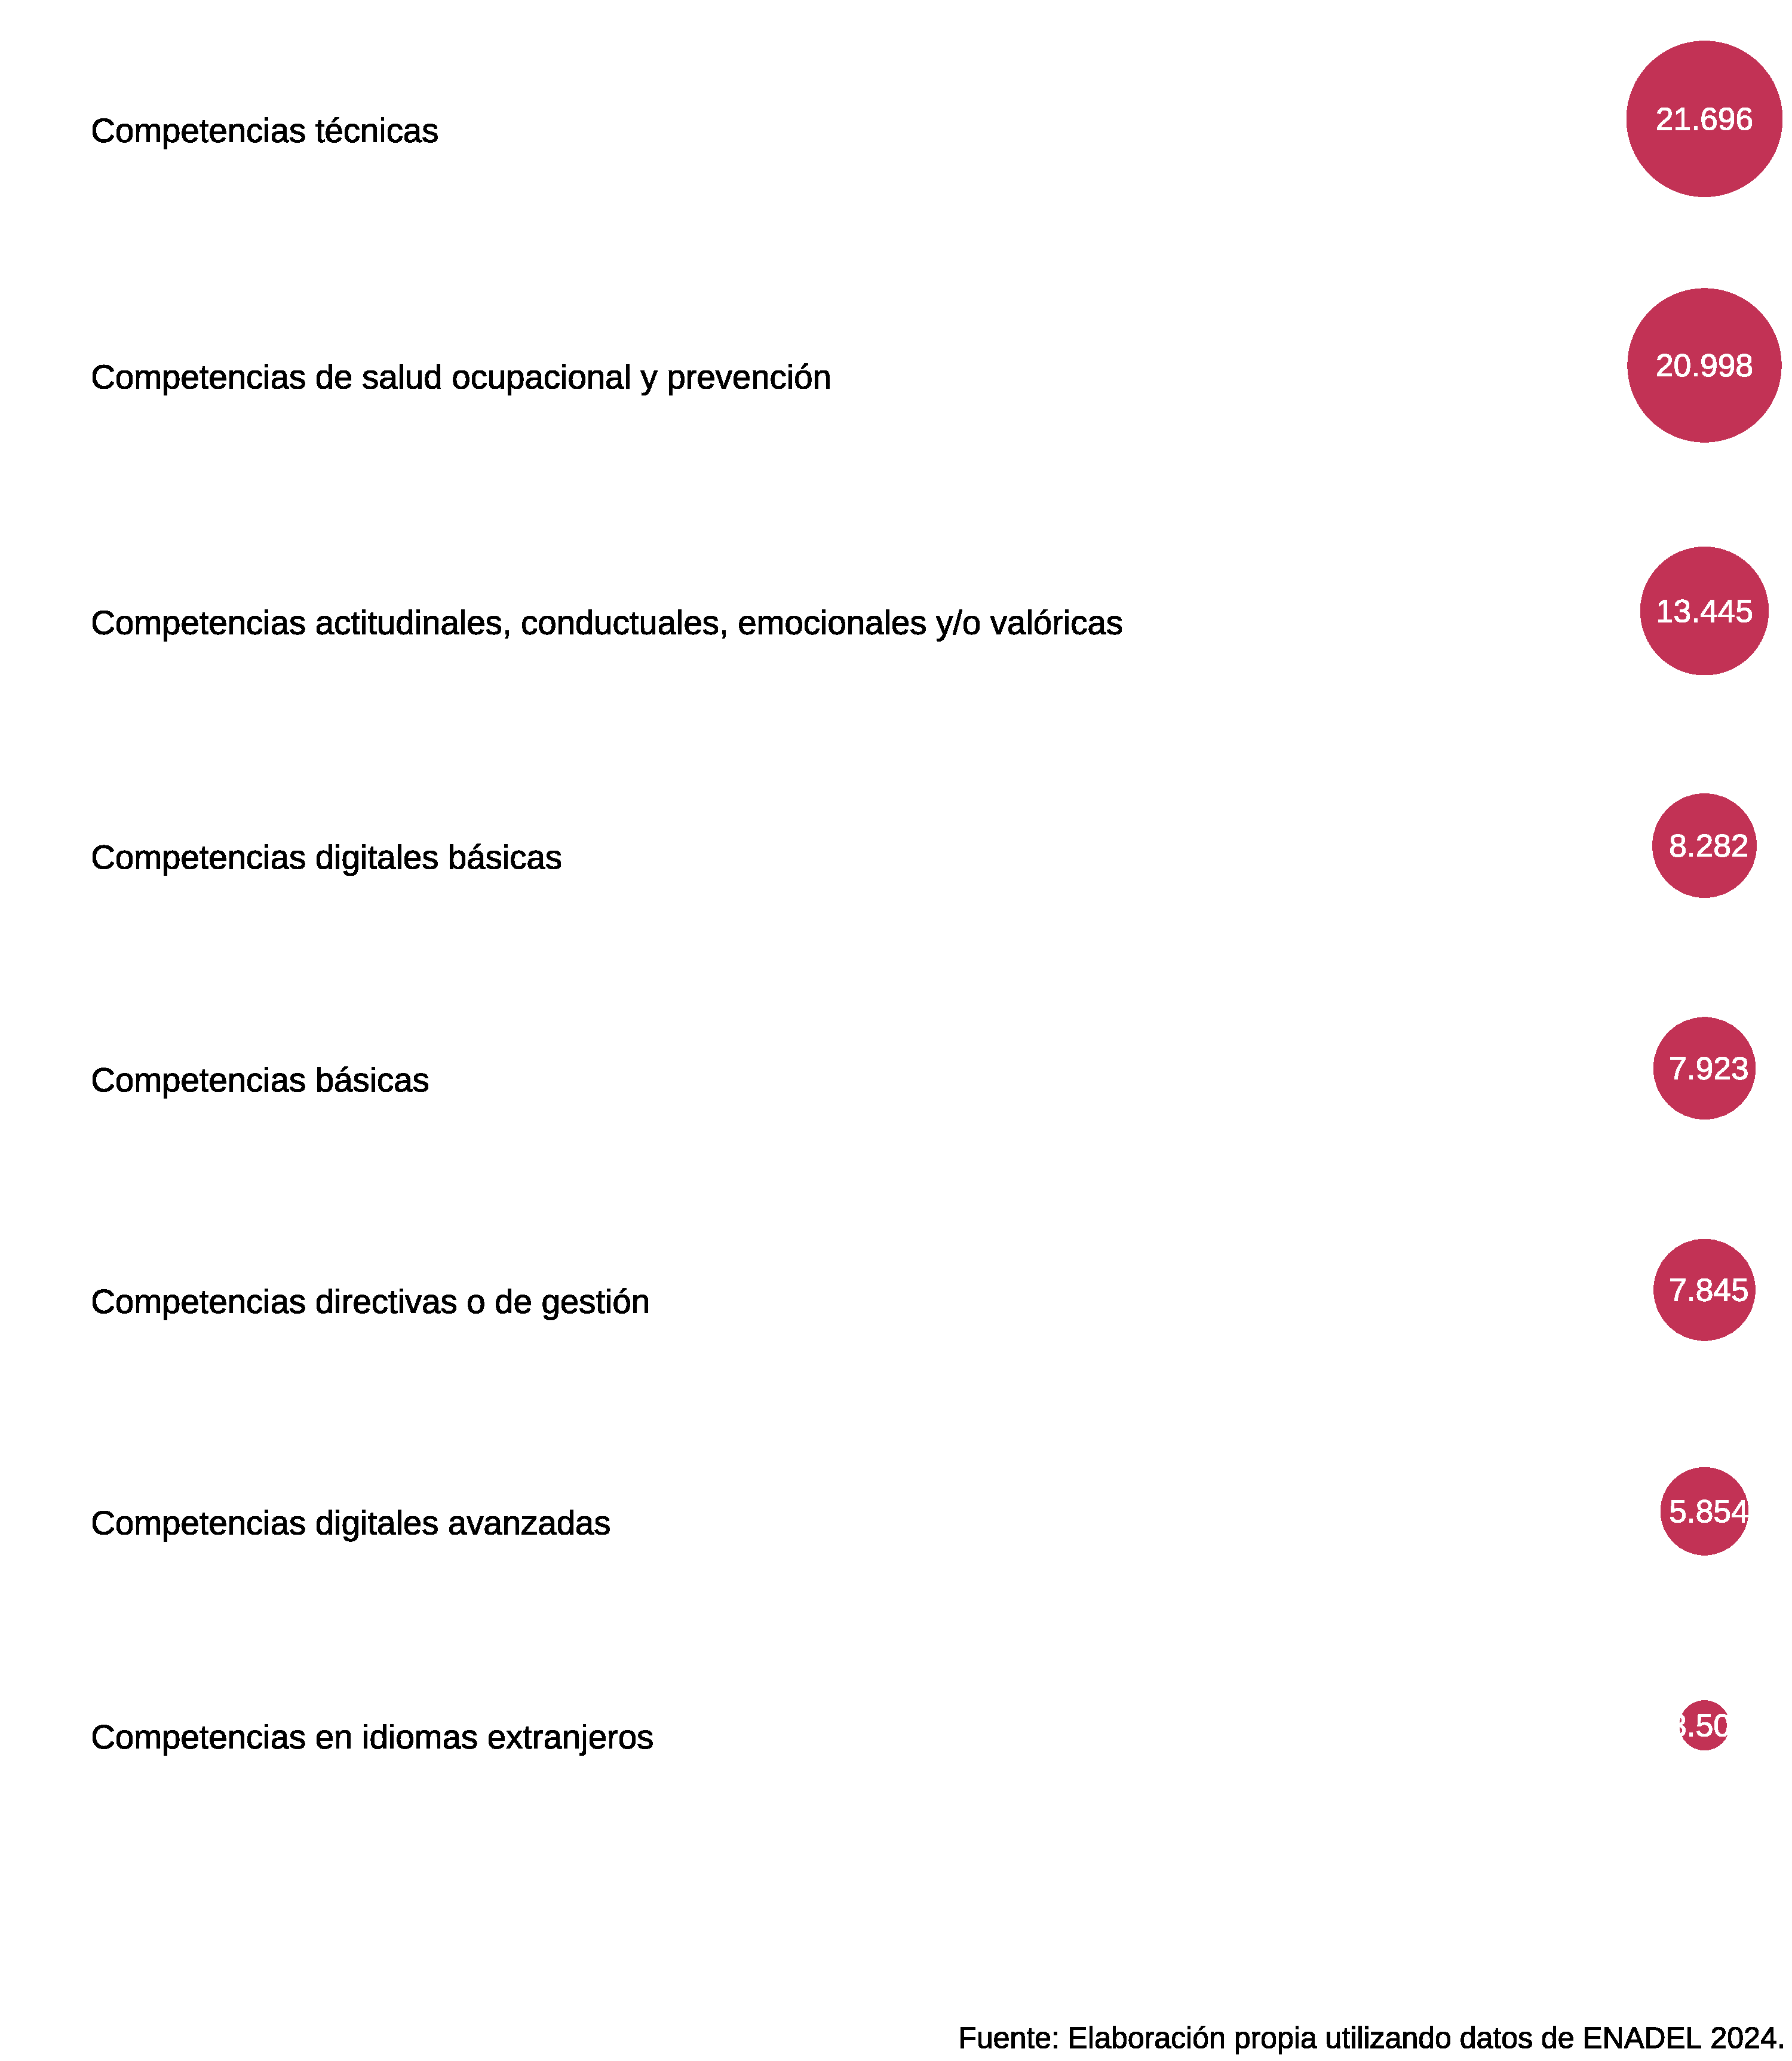
\includegraphics[width=1\textwidth,height=\textheight]{reporte_2024_files/figure-pdf/fig-competencias_necesarias-1.pdf}

}

\end{figure}%

\subsection{Fuentes de financiamiento de la
capacitación}\label{fuentes-de-financiamiento-de-la-capacitaciuxf3n}

La Figura~\ref{fig-capacitacion_finan} ilustra la cantidad de empresas
según las principales fuentes de financiamiento destinadas a la
capacitación durante los últimos doce meses. La principal fuente de
financiamiento para capacitación utilizada por las empresas corresponde
a Recursos propios de la empresa donde 117.821 organizaciones indican
utilizar esta fuente de financiamiento. En segundo lugar, 31.363
empresas indican haber utilizado Financiamiento vía franquicia
tributaria (SENCE) como principal fuente de financiamiento para sus
capacitaciones, seguido de Una mutual / Instituto de Seguridad Laboral
(ISL) ( 19.244). La fuentes de financiamiento menos utilizadas
corresponden a Programa público de capacitación (FOSIS, Mineduc,
SENCE-FONCAP u otro) ( 2.780), Recursos propios de trabajadores ( 1.639
) y Beca de institución privada ( 382).

\begin{figure}[H]

\caption{\label{fig-capacitacion_finan}Fuentes de financiamiento de la
capacitación}

\centering{

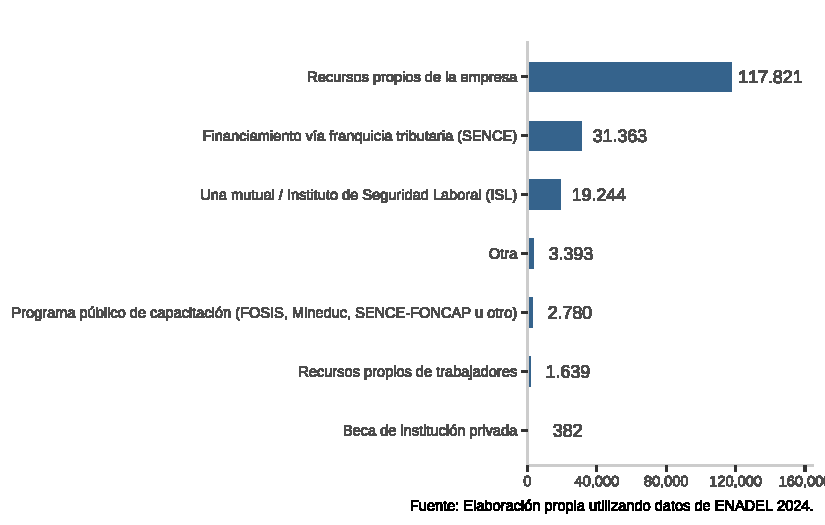
\includegraphics{reporte_2024_files/figure-pdf/fig-capacitacion_finan-1.pdf}

}

\end{figure}%

\newpage

\section{Conclusión}\label{conclusiuxf3n}

Los resultados de la ENADEL 2024 destacan importantes desafíos en el
mercado laboral chileno, especialmente en relación con las ocupaciones
de difícil cobertura. Estas dificultades se concentran principalmente en
sectores como Comercio, Alojamiento y de servicio de comida, y Comercio,
donde posiciones como Obreros de la construcción de edificios y Obreros
de explotaciones agrícolas presentan una alta demanda insatisfecha. A
nivel regional, se observan mayores dificultades en regiones como
Biobío, Los Lagos y Ñuble, mientras que las macrozonas centro-sur y sur
enfrentan importantes retos en términos de dotación de personal. Entre
las principales barreras identificadas, destacan Candidatos sin
competencias o habilidades técnicas requeridas, la Falta de postulantes,
y las Condiciones laborales (ubicación, horario y/o jornada) no
aceptadas.Asimismo, los sectores económicos más afectados evidencian una
necesidad crítica de formación y capacitación para cerrar las brechas de
habilidades y adaptarse a las demandas actuales del mercado laboral. Los
hallazgos subrayan la importancia de continuar en el fortalecimiento de
la intermediación laboral, optimizando los programas de capacitación y
promoviendo políticas públicas que impulsen una mayor equidad y
competitividad. \newpage
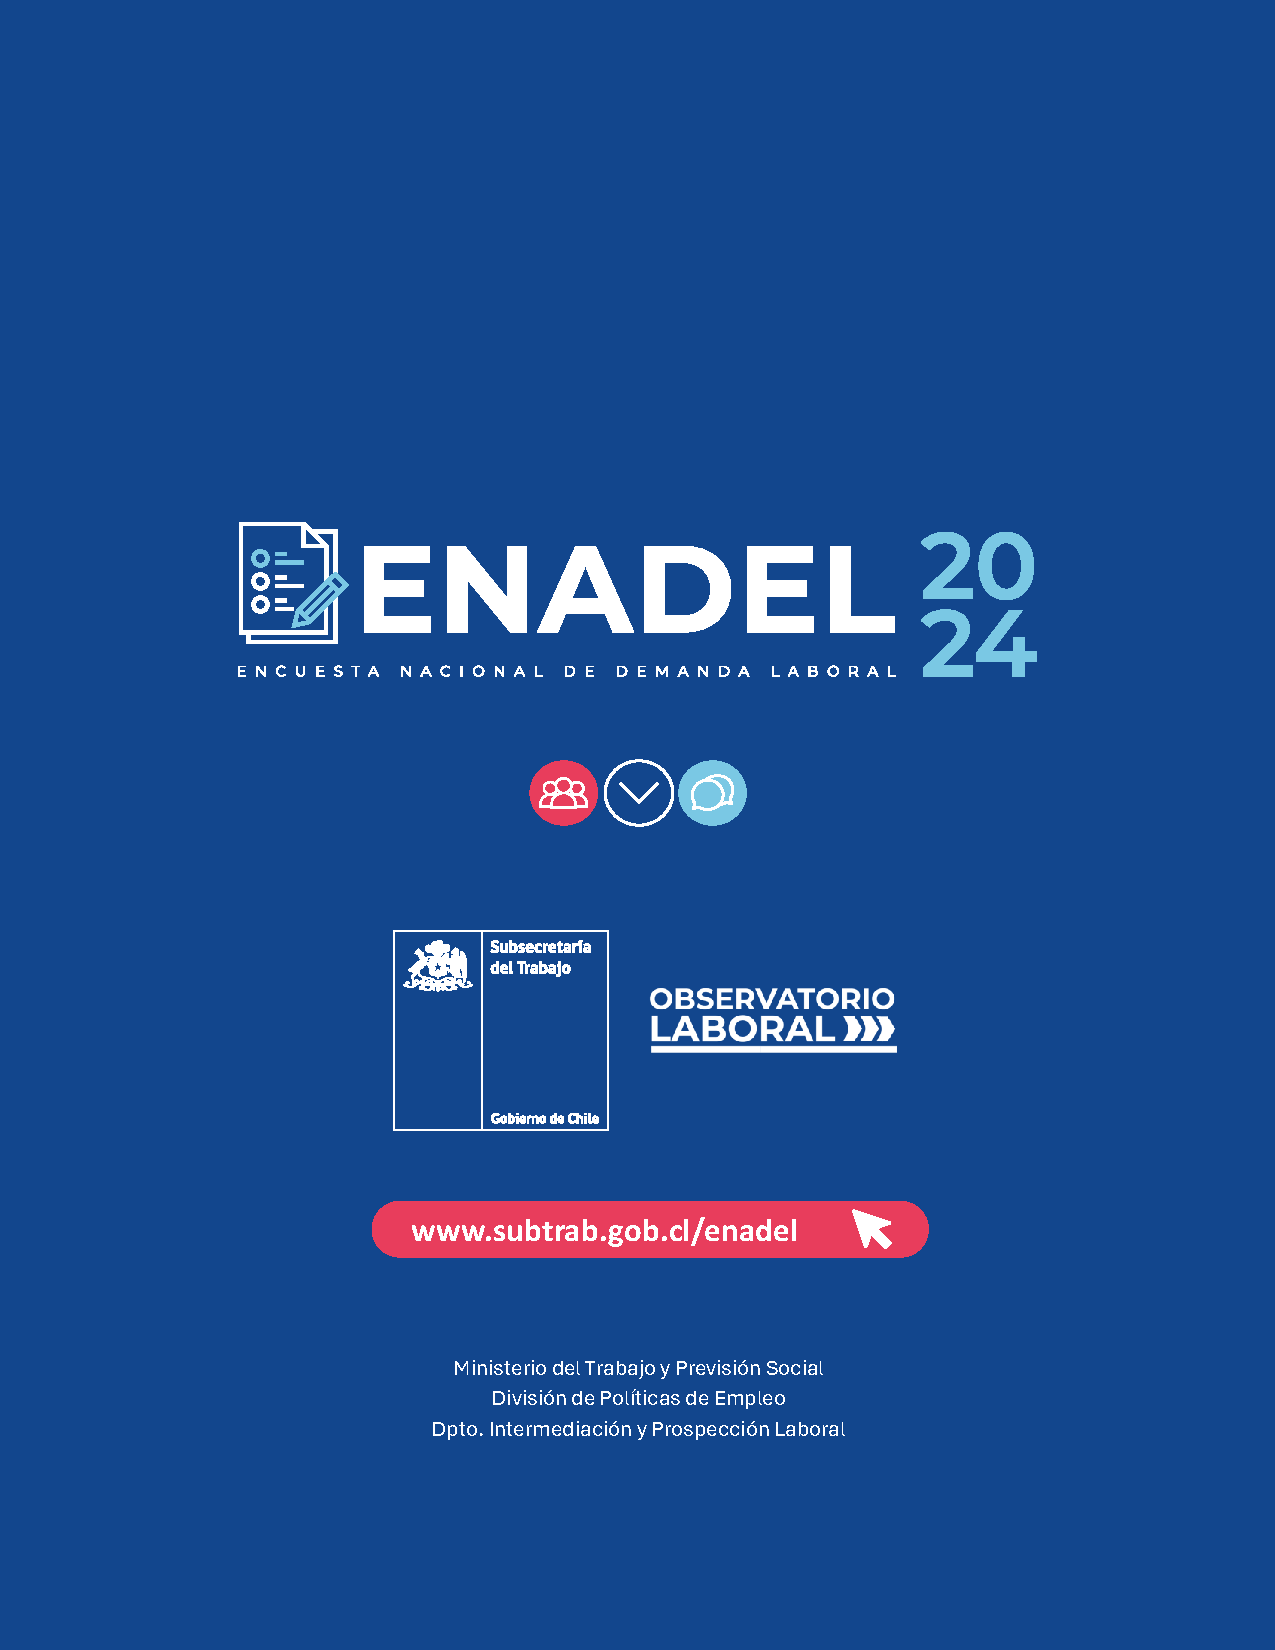
\includepdf[pages=-]{../Quarto/Portada/Contraportada Enadel 2024.pdf}




\end{document}
